\chapter{Σχεδιασμός και Υλοποίηση Αισθητήρα}
\label{ch:sensor}

\section{Εισαγωγή}

Στο συγκεκριμένο κεφάλαιο θα εξεταστεί αναλυτικά η αρχιτεκτονική και οι
αρχές λειτουργίας του συστήματος. Παρουσιάζονται τα δομικά στοιχεία με
τα χαρακτηριστικά τους, η θεωρία λειτουργίας του αισθητήρα, το
σχηματικό, οι απαιτήσεις και οι περιορισμοί του συστήματος καθώς και η
τελική πλακέτα.

\section{Δομικά Στοιχεία του Συστήματος}

\subsection{Γεννήτρια DDS}

Ο υπολογισμός της σύνθετης αντίστασης του δείγματος απαιτεί τη διέγερση
του από ένα ηλεκτρικό σήμα μέσω των ηλεκτροδίων και μίας αντίστασης
(shunt resistor) συνδεδεμένη σε σειρά. Για τη δημιουργία του σήματος
επιλέχθηκε ο DDS (Direct Digital Synthesis) AD9833. Πρόκειται για ένα
ολοκληρωμένο κύκλωμα που επιτρέπει την παραγωγή ημιτοειδών, τετραγωνικών
και τριγωνικών κυματομορφών. Επιλέχθηκε λόγω του χαμηλού κόστους και
κατανάλωσης ισχύος, αλλά και τον εύκολο έλεγχο μέσω SPI για τον
προγραμματισμό του επιθυμητού σήματος και συχνότητας μέσω του
μικροελεγκτή. Υποστηρίζει συχνότητες εξόδου από 0-12.5 MHz και παρέχει
πλάτος εξόδου περίπου 0,6Vpp. \cite{refad9833}

\begin{figure}[H]
  \centering
  \includegraphics[width=0.34\textwidth]{ad9833-dds-module.png}
  \caption{Μονάδα γεννήτριας DDS AD9833.}
  \label{fig:ad9833-module}
\end{figure}

\subsection{Ανιχνευτής Κέρδους-Φάσης}

Για τον υπολογισμό της πτώσης τάσης και της διαφοράς φάσης μεταξύ τάσης
και ρεύματος του δείγματος χρησιμοποιήθηκε η μονάδα \textbf{AD8302}.
Πρόκειται για ένα ολοκηρωμένο κύκλωμα ανίχνευσης κέρδους και φάσης
μεταξύ δύο AC σημάτων εισόδου, το οποίο παράγει στην έξοδο δύο DC τιμές
τάσεων, μία για το λόγο των πλατών και μία για τη διαφορά φάσης
αντίστοιχα. Η ευαισθησία της εξόδου είναι 30mV/db για το κέρδος και
10mV/° για τη φάση, ενώ μπορεί να δεχθεί σήματα συχνότητας έως και
2.7GHz. Παρακάτω φαίνεται το εξιδανικευμένο διάγραμμα εισόδων-εξόδου για
την εκάστοτε έξοδο. \cite{ref33}

\begin{figure}[H]
  \centering
  \includegraphics[width=0.76\textwidth]{ad8302-phase-transfer.png}
  \caption{Ιδανική χαρακτηριστική εξόδου φάσης του AD8302.}
  \label{fig:ad8302-phase-transfer}
\end{figure}

\begin{figure}[H]
  \centering
  \includegraphics[width=0.76\textwidth]{ad8302-magnitude-transfer.png}
  \caption{Ιδανική χαρακτηριστική εξόδου λόγου πλατών του AD8302.}
  \label{fig:ad8302-magnitude-transfer}
\end{figure}

Η συνάρτηση μεταφοράς της εξόδου για το λόγο των πλατών δίνεται από τη
σχέση

\[V_{MAG} = 0,9 + 0,03 \cdot \left( 20\log\frac{\left| V_{a} \right|}{\left| V_{b} \right|} \right) \tag{4.1}\]

ενώ για τη φάση ισχύει

\[V_{PHASE} = 0,9 - 0,01 \cdot \left( \Delta\varphi - 90^{\circ} \right) \tag{4.2}\]

\subsection{Μονάδα Analog-to-Digital Converter}

Για τη δειγματοληψία των τιμών εξόδου του ανιχνευτή κέρδους-φάσης
χρησιμοποιήθηκε o εξωτερικός μετατροπέας αναλογικών σε ψηφιακό σήμα
(ADC) \textbf{ADS1115} των 16bits για καλύτερη ακρίβεια. Διαθέτει
τέσσερα κανάλια εισόδου κι επικοινωνεί με το πρωτόκολλο
I\textsuperscript{2}C. \cite{ref34}

\begin{figure}[H]
  \centering
  \includegraphics[width=0.45\textwidth]{ads1115-adc-module.jpg}
  \caption{Μονάδα μετατροπέα αναλογικού σε ψηφιακό σήμα ADS1115 των 16bits.}
  \label{fig:ads1115-module}
\end{figure}

\subsection{Ολοκληρωμένα Κυκλώματα}

Για τη διαμόρφωση των αναλογικών σημάτων (signal conditioning)
επιλέχθηκε ο \textbf{AD8066} λόγω της χαμηλής του κατανάλωσης. Για την
απομόνωση των σημάτων του κυκλώματος χρησιμοποιήθηκε ο \textbf{LTC6268}
σε συνδεσμολογία ακόλουθου τάσης (voltage follower). Η επιλογή του
βασίστηκε στην εξαιρετικά χαμηλή χωρητικότητα εισόδου της τάξης των fF
και στο πολύ χαμηλό ρεύμα πόλωσης (input bias current) στην κλίμακα των
pA, προκειμένου να ελαχιστοποιηθεί η φόρτωση του δείγματος και να
αποφευχθεί η αλλοίωση των πραγματικών ηλεκτρικών χαρακτηριστικών. \cite{ref35,ref36}

Στη συνέχεια, τα παραπάνω σήματα οδηγούνται στους διαφορικούς ενισχυτές \textbf{AD8130.} Πρόκειται
για έναν high-speed διαφορικό ενισχυτή που δεν απαιτεί εξωτερικά
εξαρτήματα και προσφέρει υψηλή απόρριψη κοινού θορύβου, με περίπου -80db
στο 1MHz \cite{ref37,ref38}. Τέλος, τα δύο σήματα εξόδου από τους διαφορικούς ενισχυτές οδηγούνται
μέσω του αναλογικού διακόπτη \textbf{ADG733} εναλλάξ στη μία είσοδο του AD8302, ενώ στη δεύτερη είσοδο
υπάρχει μόνιμα το σήμα αναφοράς.

\subsection{Μικροελεγτκής}

Για τον έλεγχο και το συντονισμό της λειτουργίας του συστήματος
χρησιμοποιήθηκε ο μικροελεγκτής ESP32-NodeMCU-32s, λόγω της ευχριστίας και της εύκολης διασύνδεσης στο διαδίκτυο. Ο μικροελεγκτής
αναλαμβάνει το ρόλο του προγραμματισμού της γεννήτριας AD9833 μέσω του
πρωτοκόλλου SPI, τη λήψη των δεδομένων από τον μετατροπέα ADS1115 με το
πρωτόκολλο \(I^{2}C\), τον έλεγχο του αναλογικού διακόπτη και τέλος την
εκτέλεση των απαραίτητων πράξεων για τον υπολογισμό της σύνθετης
αντίστασης και την εκτίμηση της υγρασίας του δείγματος. \cite{refesp}

\begin{figure}[H]
  \centering
  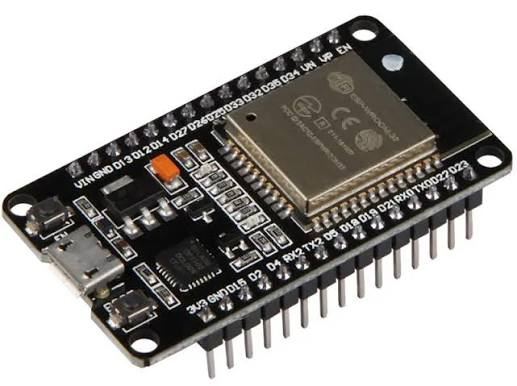
\includegraphics[width=0.40\textwidth]{figures/esp32.jpeg}
  \caption{Ο μικροελεγκτής ESP32-NodeMCU-32s που χρησιμοποιήθηκε για το σύστημα.}
  \label{fig:signal-buffering-filtering}
\end{figure}




\section{Απαιτήσεις του Συστήματος}

Μία από τις απαιτήσεις του συστήματος είναι η ανίχνευση μικρών μεταβολών
της χωρητικότητας. Σύμφωνα με τις μετρήσεις που πραγματοποιήθηκαν με τον
Αναλυτή Εμπέδησης, η διακύμανση της χωρητικότητας στα δείγματα που
εξετάστηκαν ήταν της τάξης των δεκάδων pF. Τόσο χαμηλές χωρητικότητες
μπορούν εύκολα να επισκιαστούν από παρασιτικές χωρητικότητες,
παρεμβολές, ακατάλληλο σχεδιασμό της πλακέτας και γενικότερα συστημικά
σφάλματα. Έτσι, δόθηκε ιδιαίτερη προσοχή στο σχεδιασμό προκειμένου να
ελαχιστοποιηθούν τα σφάλματα στο μέγιστο δυνατό.

Ακόμη, ένα μειονέκτημα του ανιχνευτή κέρδους-φάσης είναι η μη
γραμμικότητα των συναρτήσεων εξόδου για διαφορά φάσης από
0\textsuperscript{ο} έως +-30\textsuperscript{ο} (\figref{fig:ad8302-phase-error}). Από τον
αναλυτή εμπέδησης φάνηκε πως η φάση των δειγμάτων κυμαινόταν από τιμές
κοντά στις 0\textsuperscript{ο} έως και τις -10\textsuperscript{ο}. Για
αυτό το λόγο, δημιουργήθηκε ένα τρίτο σήμα αναφοράς Vereference με
αρκετά μεγαλύτερη διαφορά φάσης συγκριτικά με τα δύο σήματα που
λαμβάνονται από το σύστημα, προκειμένου να μειωθεί το σφάλμα εξόδου.
Εφόσον ληφθεί η μέτρηση του κάθε σήματος αναφορικά με το Vreference,
γίνεται μαθηματικά η απαλοιφή του Vreference μέσω του μικροελεγκτή και
εξάγεται το τελικό V\textsubscript{MAG} και V\textsubscript{PHASE} των
δύο σημάτων ενδιαφέροντος.

\begin{figure}[H]
  \centering
  \includegraphics[width=0.6\textwidth]{ad8302-phase-error.png}
  \caption{Χαρακτηριστική εξόδου φάσης και σφάλματος του AD8302 συναρτήσει της διαφοράς φάσης. \cite{ref33}}
  \label{fig:ad8302-phase-error}
\end{figure}

\section{Προσέγγιση και Μεθοδολογία}

Η μεθοδολογία που χρησιμοποιείται από τον αισθητήρα 
βασίζεται στον υπολογισμό των ηλεκτρικών μεγεθών που
χαρακτηρίζουν το δείγμα. Για την εκτίμηση αυτή, ο
αισθητήρας παράγει μία ημιτονοειδή κυματομορφή για να
διεγείρει το δείγμα το οποίο έχει τοποθετηθεί σε σειρά
με μια αντίσταση. Τα σήματα από τα δύο άκρα των στοιχείων
λαμβάνονται μέσω ακολούθων τάσεων και οδηγούνται σε δύο
διαφορικούς ενισχυτές, ένα για το κάθε στοιχείο, προκειμένου
να υπολογιστεί διαφορικά η πτώση τάσης αλλά και η διαφορά φάσης
μεταξύ των δύο στοιχείων. Από τις παραπάνω πληροφορίες, μπορούν
στη συνέχεια να υπολογιστούν όλα τα ηλεκτρικά μεγέθη που χρειάζονται
για την υλοποίηση του συστήματος.
\par Στο Σχήμα 4.7 παρουσιάζεται το σχηματικό της προσομοίωσης της
πειραματικής διάταξης μέσω LTSpice για ένα δοκιμαστικό δείγμα με τιμές
300Ω και 150p. Στο Σχήμα 4.8 φαίνεται
η πτώση τάσης και η διαφορά φάσης μεταξύ του δείγματος και της
αντίστασης, η οποία χρησιμοποιείται για τη λήψη των μετρήσεων του
ρεύματος του κυκλώματος. Τελικά, μπορεί να εξαχθεί η σχέση 
τάσης και ρεύματος του δείγματος όπως θα αναλυθεί παρακάτω.

\begin{figure}[H]
  \centering
  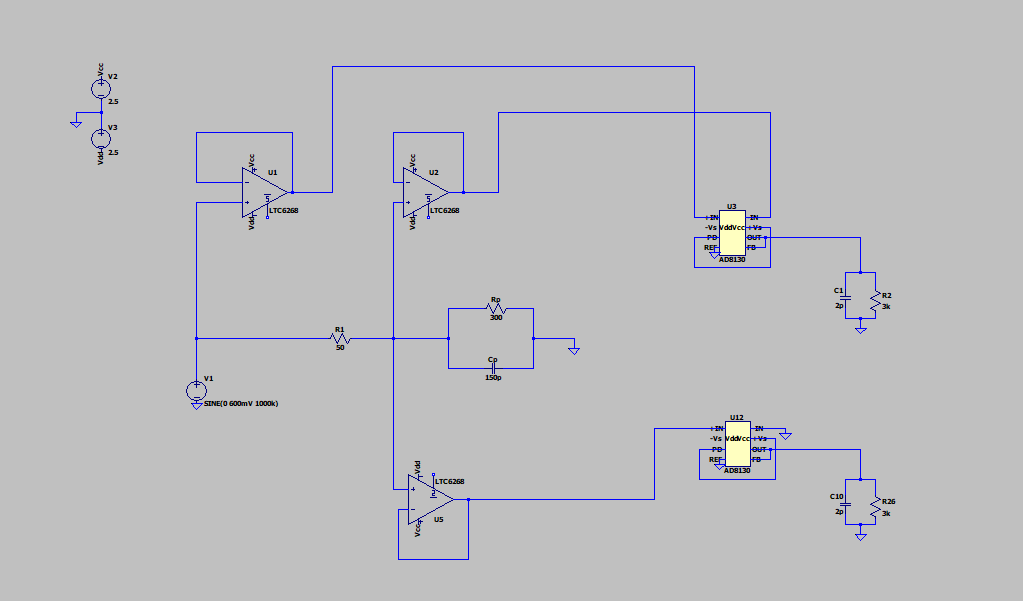
\includegraphics[width=0.99\textwidth]{figures/ad8130.png}
  \caption{Μέτρηση της πτώσης τάσης και διαφοράς φάσης στα στοιχεία με τη χρήση διαφορικού ενισχυτή. Ο παραλληλισμός R=3k και C=2pF προσομοιώνει την είσοδο της επόμενης βαθμίδας, του AD8302.}
  \label{fig:lt}
\end{figure}


\begin{figure}[H]
  \centering
  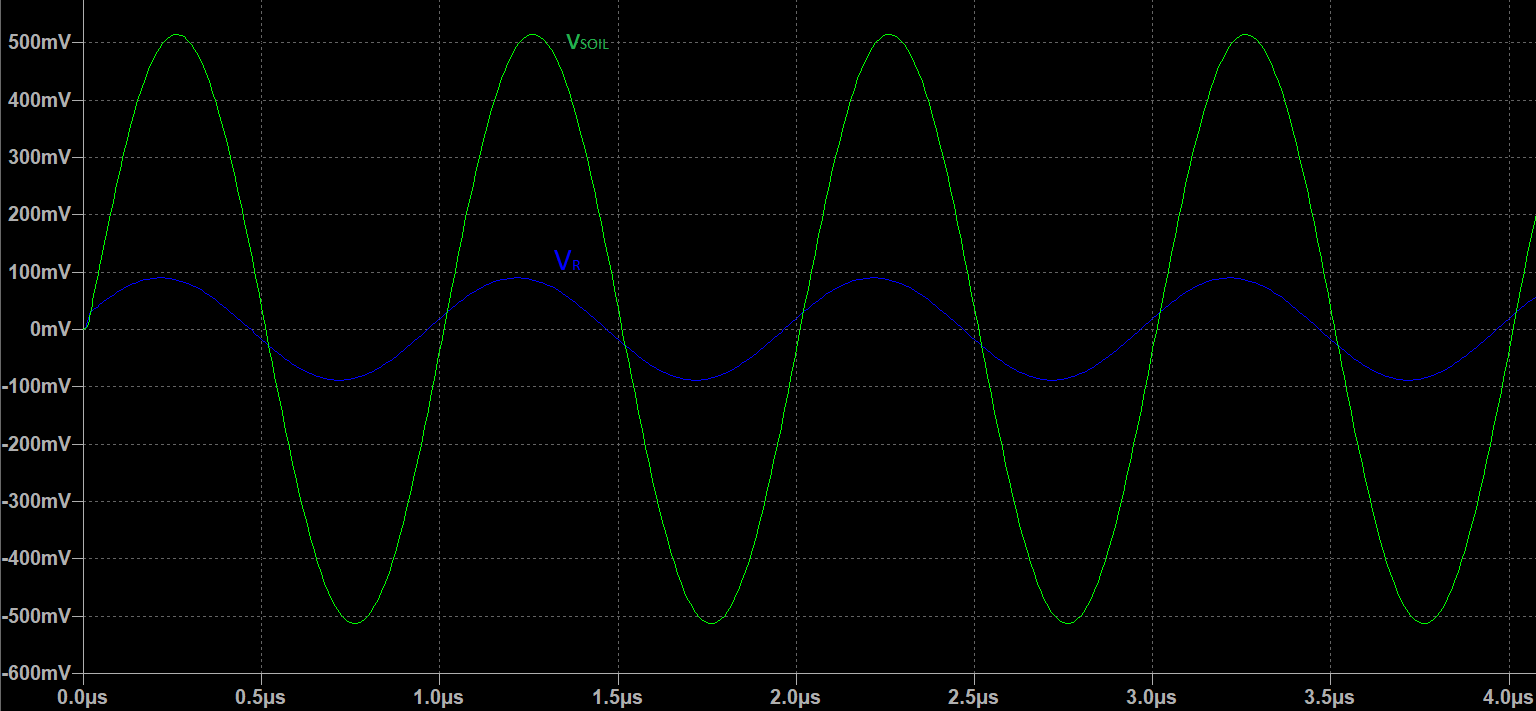
\includegraphics[width=0.9\textwidth]{figures/spice.png}
  \caption{Προσομοίωση αποτελεσμάτων της πτώσης τάσεως και της διαφοράς φάσης μεταξύ δείγματος και αντίστασης αναφοράς..}
  \label{fig:sensor-architecture}
\end{figure}




Στο \figref{fig:sensor-architecture} φαίνεται η συνολική αρχιτεκτονική του συστήματος. Αρχικά,
ο DDS παράγει ένα ημιτονοειδές σήμα συχνότητας 1MHz και πλάτους 0,6mVpp,
το οποίο περιλαμβάνει μία DC συνιστώσα (DC offset). Ωστόσο, επειδή μία
DC συνιστώσα θα προκαλούσε οξείδωση στα ηλεκτρόδια λόγω της
ηλεκτρόλυσης, το σήμα θα πρέπει να είναι καθαρά εναλλασσόμενο (AC). Για
αυτό το λόγο, στην έξοδο του DDS έχει τοποθετηθεί ένα υψηπερατό φίλτρο
όπως φαίνεται στο \figref{fig:dds-high-pass-filter} με συχνότητα αποκοπής

\[f = \frac{1}{2\pi * R_{21} * C_{34}} = \frac{1}{2\pi * 1k * 0.1u} = 1.6kHz \tag{4.3}\]

\begin{figure}[H]
  \centering
  \includegraphics[width=0.9\textwidth]{sensor-system-architecture.png}
  \caption{Συνολική αρχιτεκτονική του συστήματος.}
  \label{fig:sensor-architecture}
\end{figure}

\begin{figure}[H]
  \centering
  \includegraphics[width=0.99\textwidth]{dds-high-pass-filter.png}
  \caption{Η μονάδα παραγωγής σημάτων και το υψηπερατό φίλτρο}
  \label{fig:dds-high-pass-filter}
\end{figure}

Στη συνέχεια, για τη βελτίωση του SNR το σήμα ενισχύεται μέσω ενός
τελεστικού σε συνδεσμολογία αναστρέφοντα ενισχυτή με κέρδος

\[A_{v} = - \ \frac{R_{14}}{R_{13}} = \  - \ \frac{10k}{6.8k} = - 1.5 \tag{4.4}\]

Το σήμα αυτό χρησιμοποιείται για τη διέγερση του δείγματος αλλά και την
παραγωγή του σήματος αναφοράς, οπότε και στέλνεται μέσω του All Pass
φίλτρου για τη δημιουργία καθυστέρησης φάσης περίπου \(35^{\circ}\) σε σχέση
με το αρχικό σήμα (\figref{fig:excitation-reference-conditioning}).

\begin{figure}[H]
  \centering
  \includegraphics[width=0.88\textwidth]{excitation-reference-conditioning.png}
  \caption{Η διαμόρφωση των σημάτων διέγερσης και αναφοράς. Ο άνω τελεστικός λειτουργεί ως αναστρέφων ενισχυτής ενώ ο κάτω τελεστικός σε συνδεσμολογία All Pass Filter εισάγει τη διαφορά φάσης.}
  \label{fig:excitation-reference-conditioning}
\end{figure}

Κατά την εφαρμογή του σήματος διέγερσης στο δείγμα και την αντίσταση
αναφοράς (R10), τα σήματα στα άκρα των δύο στοιχείων λαμβάνονται μέσω
κυκλωμάτων απομόνωσης (buffers) τα οποία διαθέτουν πολύ υψηλή αντίσταση
αλλά χαμηλή χωρητικότητα εισόδου (Σχήμα 4.12). Στη συνέχεια, οδηγούνται
στους διαφορικούς ενισχυτές για τον υπολογισμό της πτώσης τάσεων στα δύο
στοιχεία (\figref{fig:differential-amplifiers-switching}).

\begin{figure}[H]
  \centering
  \includegraphics[width=0.82\textwidth]{signal-buffering-filtering.png}
  \caption{Οι τελεστικοί στα άκρα της αντίστασης και του δείγματος σε συνδεσμολογία ακολούθου τάσης και τα χαμηλοπερατά φίλτρα στις εξόδους τους.}
  \label{fig:signal-buffering-filtering}
\end{figure}

Τα δύο σήματα εξόδου των διαφορικών ενισχυτών, οδηγούνται σε έναν
αναλογικό διακόπτη, ο οποίος ελέγχεται από μία έξοδο (GPIO) του ESP32.
Τελικά, στην είσοδο του ανιχνευτή κέρδους φάσης καταλήγει το σήμα
αναφοράς και, εναλλάξ, τα δύο σήματα που επιλέγονται από τον
διακόπτη προκειμένου να πραγματοποιηθεί η μέτρηση για το κάθε στοιχείο
ξεχωριστά (\figref{fig:differential-amplifiers-switching}). Η έξοδος του ανιχνευτή δειγματοληπτείται από τον
εξωτερικό μετατροπέα αναλογικού σε ψηφιακό ώστε να γίνουν οι απαραίτητοι
υπολογισμοί μέσω του μικροελεγκτή για την εξαγωγή των ηλεκτρικών
παραμέτρων του δείγματος (\figref{fig:phase-gain-detector-adc})

\begin{figure}[H]
  \centering
  \includegraphics[width=0.6\textwidth]{differential-amplifiers-switching.png}
  \caption{Τα σήματα οδηγούνται στους  διαφορικικούς ενισχυτές όπου μέσω δύο χαμηλοπερατών φίλτρων παιρνούν στον αναλογικό διακόπτη.}
  \label{fig:differential-amplifiers-switching}
\end{figure}

\begin{figure}[H]
  \centering
  \includegraphics[width=0.7\textwidth]{phase-gain-detector-adc.png}
  \caption{Τα σήματα οδηγούνται στον ανιχνευτή κέρδους-τάσης και στη συνέχεια οι έξοδοι του διαβάζονται από τον ADC.}
  \label{fig:phase-gain-detector-adc}
\end{figure}


Το σχηματικό του ολοκληρωμένου συστήματος εμφανίζεται στο Σχήμα 4.15

\begin{figure}[H]
  \centering
  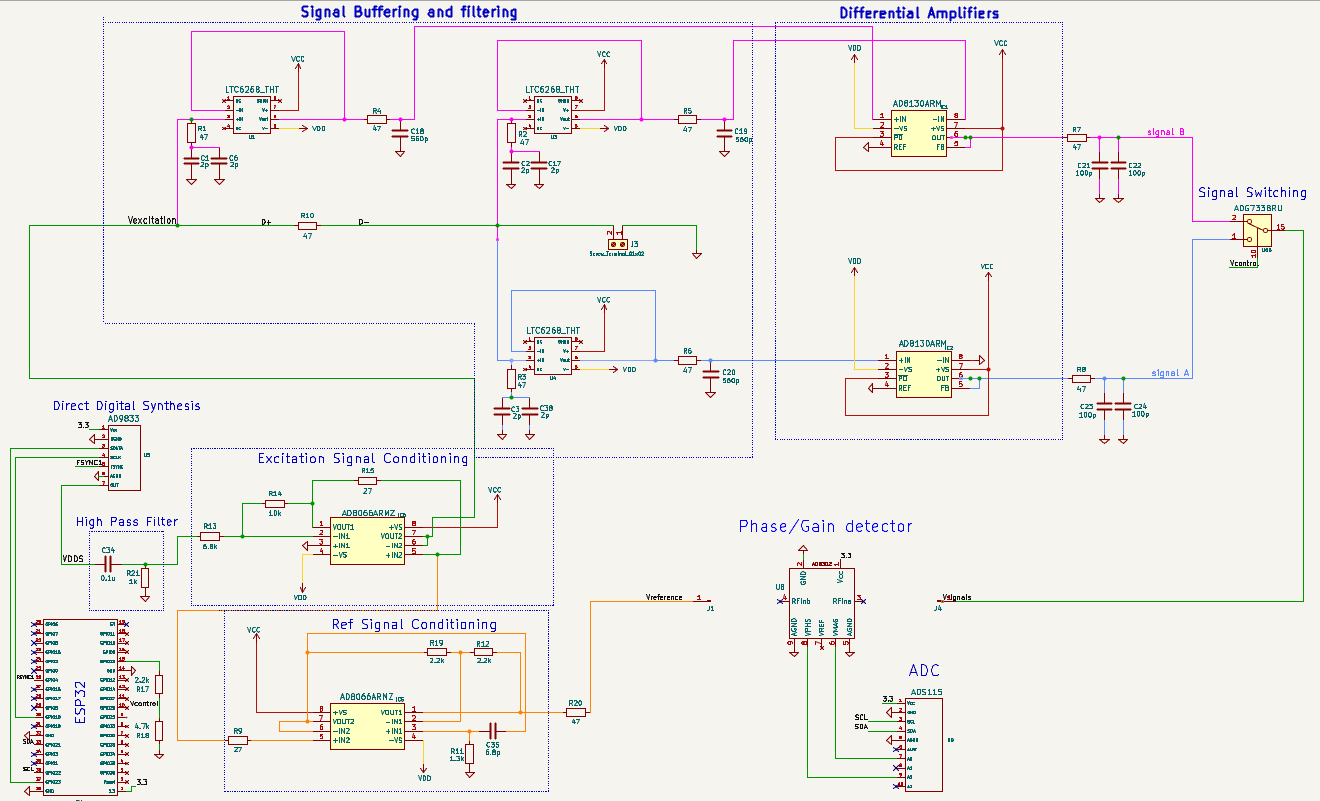
\includegraphics[width=1\textwidth]{figures/whole.png}
  \caption{Απεικόνιση του σχηματικού του κυκλώματος με όλες τις επιμέρους βαθμίδες .}
  \label{fig:phase-gain-detector-adc}
\end{figure}



Έστω ότι ορίζουμε ως \(V_{A}\) τη διαφορά τάσης στα άκρα των
ηλεκτροδίων, \(V_{B}\) τη διαφορά τάσης στα άκρα της αντίστασης και
\(V_{ref}\) το διαμορφωμένο σήμα με καθυστέρηση φάσης \(35^{\circ}\). Ως \(\left|\Delta\varphi_{1}\right|\) ορίζεται το μέτρο της διαφοράς φάσης μεταξύ  \(V_{A}\) και του σήματος αναφοράς \(V_{ref}\) . Αντίστοιχα, ως \(\left|\Delta\varphi_{2}\right|\) ορίζεται το μέτρο της διαφοράς φάσης μεταξύ  \(V_{B}\) και του \(V_{ref}\) . Μετά
από δύο εναλλαγές του διακόπτη, μετρώνται τα παρακάτω ζεύγη μεγεθών

\[
V_{\mathrm{MAG}1}=0{,}9+0{,}03\left(20\log_{10}
\frac{\left|V_{A}\right|}{\left|V_{ref}\right|}\right)
\tag{4.5}\]

\[
V_{\mathrm{PHASE}1}
=
0{,}9
-
0{,}01
\left(
\left|\Delta\varphi_{1}\right|
-
90^{\circ}
\right)
\tag{4.6}
\]

και

\[
V_{\mathrm{MAG}2}=0{,}9+0{,}03\left(20\log_{10}
\frac{\left|V_{B}\right|}{\left|V_{ref}\right|}\right)
\tag{4.7}
\]

\[
V_{\mathrm{PHASE}2}
=
0,9
-
0,01
\left(
\left|\Delta\varphi_{2}\right|
-
90^{\circ}
\right)
\tag{4.8}
\]

Για τη σχέση (4.5), ισχύει

\[
\log_{10}\left(\frac{\left|V_{A}\right|}{\left|V_{ref}\right|}\right)
=\frac{V_{\mathrm{MAG}1}-0{,}9}{0{,}6}
\tag{4.9}\]

και επομένως

\[
\left|V_{A}\right|=
10^{\frac{V_{\mathrm{MAG}1}-0{,}9}{0{,}6}}\left|V_{ref}\right|
\tag{4.10}
\]

Ενώ αντίστοιχα για το \(V_{B}\) ισχύει

\[
\left|V_{B}\right|=
10^{\frac{V_{\mathrm{MAG}2}-0{,}9}{0{,}6}}\left|V_{ref}\right|
\tag{4.11}
\]

Για να βρεθεί ο λόγος των πλατών, διαιρούνται κατά μέλη οι σχέσεις 4.10
και 4.11 και προκύπτει τελικά

\[
\frac{\left|V_{A}\right|}{\left|V_{B}\right|}
=10^{\frac{V_{\mathrm{MAG}1}-V_{\mathrm{MAG}2}}{0{,}6}}
\tag{4.12}
\]

Από τις σχέσεις 4.6 και 4.8 υπολογίζονται αντίστοιχα οι διαφορές φάσης

\[
\left|\Delta\varphi_{1}\right|
=\frac{0{,}9-V_{\mathrm{PHASE}1}}{0{,}01}+90^{\circ}
\tag{4.13}
\]

και

\[
\left|\Delta\varphi_{2}\right|
=\frac{0{,}9-V_{\mathrm{PHASE}2}}{0{,}01}+90^{\circ}.
\tag{4.14}
\]

Η διαφορά φάσης των δύο σημάτων ενδιαφέροντος προκύπτει με απαλοιφή της κοινής φάσης του σήματος αναφοράς. Θεωρώντας ότι το σήμα αναφοράς προηγείται κατά περίπου \(35^\circ\) από τα άλλα δύο και γνωρίζοντας πως το δείγμα έχει χωρητική συμπεριφορά, ισχύει \(\varphi_3 > \varphi_2 > \varphi_1\) και έχουμε:

\[
\Delta\varphi_1 = \varphi_1 - \varphi_3 < 0
\tag{4.15}\]

\[
\Delta\varphi_2 = \varphi_2 - \varphi_3 < 0
\tag{4.16}\]

όπου \(\varphi_3\) είναι η φάση του σήματος αναφοράς.

\[
|\Delta \phi| = |\Delta \phi_2| - |\Delta \phi_1|
= (\phi_3 - \phi_2) - (\phi_3 - \phi_1)
= \phi_1 - \phi_2
= \frac{V_{\mathrm{PHASE}_1} - V_{\mathrm{PHASE}_2}}{0.01}
\tag{4.17}\]

Θεωρώντας \(Z_{\mathrm{ref}}\) για την αντίσταση αναφοράς, το ίδιο ρεύμα διαρρέει την αντίσταση αναφοράς και το δείγμα. Επομένως, η σύνθετη αντίσταση του δείγματος υπολογίζεται ως

\[
\begin{aligned}
\vec{Z}
&=\frac{\vec{V}_{A}}{\vec{I}}
 =\frac{\vec{V}_{A}}{\vec{V}_{B}/R}
 =R\frac{\vec{V}_{A}}{\vec{V}_{B}} \\
&=R\frac{\left|V_{A}\right|}{\left|V_{B}\right|}
  \angle\left(\varphi_{1}-\varphi_{2}\right) \\
&=R\,10^{\frac{V_{\mathrm{MAG}1}-V_{\mathrm{MAG}2}}{0{,}6}}
  \angle\left(\frac{V_{\mathrm{PHASE}1}-V_{\mathrm{PHASE}2}}{0{,}01}\right).
\end{aligned}
\tag{4.18}\]

Για την εξαγωγή των παραμέτρων του παράλληλου ισοδύναμου
\(R_{p}\)-\(C_{p}\), χρησιμοποιείται η μιγαδική αγωγιμότητα

\[
\begin{aligned}
\vec{Y}
&=\frac{1}{\vec{Z}}
 =\frac{1}{\left|Z\right|e^{j\varphi}} \\
&=\frac{1}{\left|Z\right|}
  \left(\cos\varphi-j\sin\varphi\right).
\end{aligned}
\tag{4.19}
\]

Από το Κεφάλαιο 3 θεωρώντας ως ηλεκτρικό ισοδύναμο το παράλληλο Rp-Cp, ισχύει επίσης

\[
\vec{Y}=\frac{1}{R_{p}}+j\omega C_{p}=G+jB,
\tag{4.20}
\]

όπου \(\omega=2\pi f\). Εξισώνοντας το πραγματικό και το φανταστικό μέρος
των σχέσεων 4.19 και 4.20, προκύπτουν

\[
G=\frac{1}{R_{p}}=\frac{\cos\varphi}{\left|Z\right|},
\qquad
B=\omega C_{p}=-\frac{\sin\varphi}{\left|Z\right|}.
\tag{4.21}
\]

Τελικά, οι παράμετροι του ισοδύναμου κυκλώματος δίνονται από τις σχέσεις


\[
R_{p}=\frac{\left|Z\right|}{\cos\varphi},
\qquad
C_{p}=-\frac{\sin\varphi}{\omega\left|Z\right|}.
\tag{4.22}
\]

Για τον υπολογισμό του πραγματικού και φανταστικού μέρους της ηλεκτρικής διαπερατότητας, ισχύει ότι 

\[
G = k_g \sigma
, \qquad
B = k_g \omega \varepsilon_0 \varepsilon_r'
\tag{4.23}\]

Δεδομένου ότι 

\[ \sigma = \omega \varepsilon_0 \varepsilon_r''\tag{4.24} \]

προκύπτει τελικά για το παράλληλο ισοδύναμο ότι 

\[
\varepsilon_r'' = \frac{1}{R_p k_g \omega \varepsilon_0} 
, \qquad
\varepsilon_r'= \frac{C_p}{k_g \varepsilon_0} 
\tag{4.25}\]

\section{Τυπωμένο Κύκλωμα}

Μετά τον έλεγχο και τη βελτιστοποίηση του συστήματος που σχεδιάστητκε στο ράστερ όπως φαίνεται στο Σχήμα 4.14, ακολούθησε η σχεδίαση του τυπωμένου κυκλώματος για τη σταθερότερη λήψη μετρήσεων, τη μείωση των ανεπιθύμητων χωρητικοτήτων, αλλά και την ελάττωση του θορύβου.


\begin{figure}[H]
  \centering
  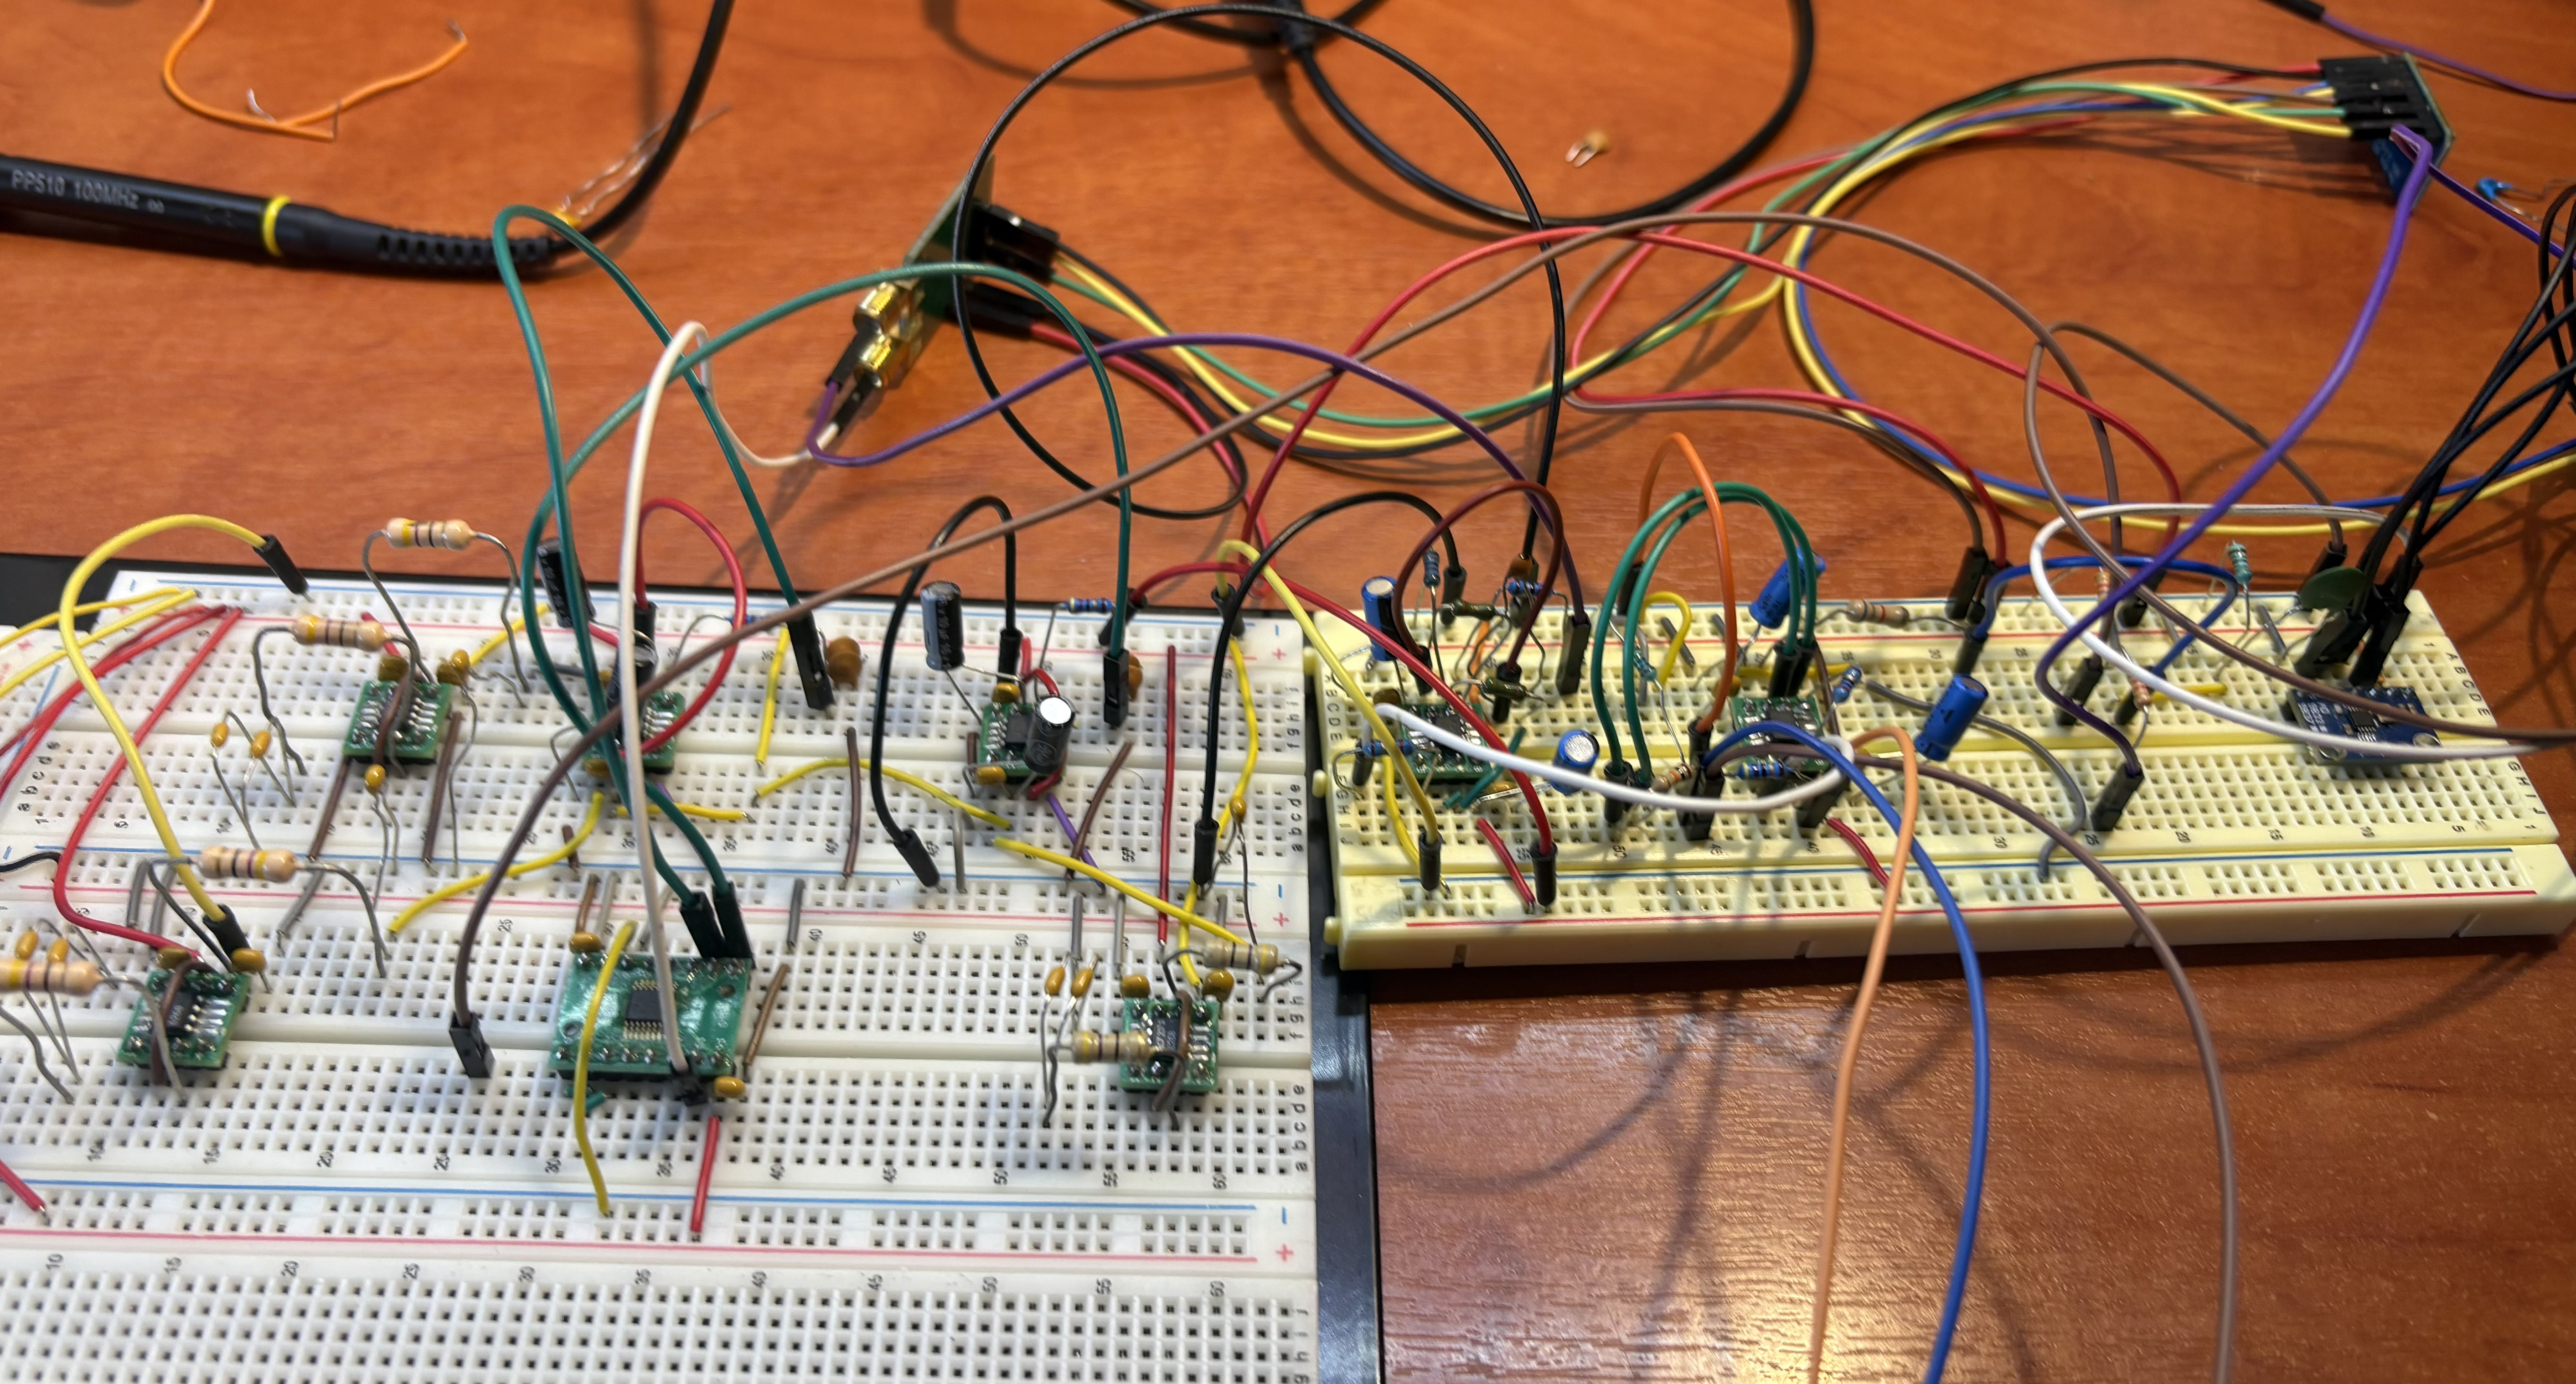
\includegraphics[width=0.9\textwidth]{figures/raster.jpg}
  \caption{Στιγμιότυπο από την πειραματική υλοποίηση του κυκλώματος σε breadboard. }
  \label{fig:signal-buffering-filtering}
\end{figure}


Η πλακέτα σχεδιάστηκε με τη χρήση του λογισμικού Kicad. Πρόκειται για πλακέτα διπλής όψεος με διαστάσεις περίπου 10cm x 17cm (Σχήμα 4.12). Τα σήματα διατηρήθηκαν όσο ήταν εφικτό στο άνω επίπεδο, προκειμένου το κάτω επίπεδο που ορίστηκε ως η γείωση να παραμείνει όσο το δυνατόν πιο συνεχές. Αυτό εξασφαλίζει την ομαλή διαδρομή των ρευμάτων επιστροφής, με αποτέλεσμα να  περιορίζεται η ηλεκτρομαγνητική σύζευξη κι ο θόρυβος.
\par Τα αναλογικά σήματα συγκεντρώθηκαν στην αριστερή μεριά της πλακέτας, ενώ τα ψηφιακά τοποθετήθηκαν στα δεξιά για να αποφευχθούν ανεπιθύμητες συζεύξεις (crosstalk). Τα σήματα που οδηγούνται στο διαφορικό ενισχυτή σχεδιάστηκαν ως διαφορικό ζεύγος (differential pair), με στόχο τη συμμετρία των δύο διαδρομών ώστε ο διαφορικός ενισχυτής να αξιοποιεί τη δυνατότητα απόρριψης του κοινού θορύβου (common-mode rejection).
\par Τέλος, η μονάδα AD8302 διαθέτει εισόδους SMA, επομένως για τη μεταφορά των σημάτων από την πλακέτα στη μονάδα ανίχνευσης κέρδους-φάσης χρησιμοποιήθηκαν U.FL connectors και καλώδια U.FL-SMA. Επιπλέον, τα καλώδια αυτά διαθέτουν εξωτερική θωράκιση η οποία συνδέθηκε στη γείωση του κυκλώματος για τον περιορισμό της επίδρασης ανεπιθύμητων ηλεκτρομαγνητικών παρεμβολών.

\begin{figure}[H]
  \centering
  \includegraphics[width=0.9\textwidth]{SoilBoard.png}
  \caption{Το προσχέδιο της πλακέτας από το λογισμικό σχεδίασης. }
  \label{fig:signal-buffering-filtering}
\end{figure}

Τα ολοκληρωμένα κυκλώματα είναι τύπου SMD, ενώ τα υπόλοιπα στοιχεία είναι through hole. Οι μονάδες AD8302, ADS1115 και AD9833 τροφοδοτούνται με 3.3V από τον ESP32. Οι γραμμές τροφοδοσίας των υπόλοιπων ολοκληρωμένων κυκλωμάτων είναι στα +2.5V και -2.5V ενώ ο ESP32 τροφοδοτείται με 5V. Τα ίχνη των γραμμών τροφοδοσίας έχουν πλάτος 1mm, μεγαλύτερο από εκείνο των γραμμών αναλογικών σημάτων, ώστε να μειώνεται η αντίσταση των διαδρομών και η πτώση τάσης, καθώς οι γραμμές τροφοδοσίας διαρρέονται από μεγαλύτερα ρεύματα.
\par Στις τροφοδοσίες των ολοκληρωμένων τοποθετήθηκαν κεραμικοί πυκνωτές αποσύζευξης (decoupling capacitors) με τιμές 0.1 uF και 10 uF όσο το δυνατόν πιο κοντά στους ακροδέκτες. Οι πυκνωτές αυτοί συμβάλλουν στη διασφάλιση σταθερής τροφοδοσίας, καθώς οι πυκνωτές των 0.1 uF καταστέλλουν κυρίως διακυμάνσεις υψηλής συχνότητας, ενώ οι 10 uF λειτουργούν ως τοπικές αποθήκες ενέργειας περιορίζοντας τις διακυμάνσεις χαμηλότερων συχνοτήτων.

\par Τέλος, για την παροχή τροφοδοσίας και  τη διασύνδεση των ηλεκτροδίων με την πλακέτα επιλέχθηκε ένας απλός διπολικός ακροδέκτης (2-terminal connector) με βήμα 5mm. 

\par Στο Σχήμα 4.18 παρουσιάζεται η τελική μορφή της πλακέτα με το σύνολο των ηλεκτρονικών εξαρτημάτων τοποθετημένα σε αυτήν.



\begin{figure}[H]
  \centering
  \includegraphics[width=0.83\textwidth]{soil.jpg}
  \caption{Η τελική μορφή της πλακέτας.}
  \label{fig:signal-buffering-filtering}
\end{figure}









\chapter{Πειραματική Αξιολόγηση και Βαθμονόμηση του Αισθητήρα}
\label{ch:calibration}

\section{Εισαγωγή}
Μετά την ολοκλήρωση της σχεδίασης και της κατασκευής της πλακέτας, καθώς και την επιβεβαίωση της ορθής λειτουργίας της με γνωστά στοιχεία R και C, ακολούθησε η πειραματική μελέτη της συμπεριφοράς του αισθητήρα σε διαφορετικά επίπεδα υγρασίας. Μέσω της λήψης και επεξεργασίας των πειραματικών δεδομένων, διερευνήθηκε η σχέση μεταξύ της απόκρισης του αισθητήρα και της υγρασίας, από όπου έγινε η εξαγωγή της χαρακτηριστικής καμπύλης και της αντίστοιχης εξίσωσης βαθμονόμησης.


\section{Ηλεκτρόδια}
Τα ηλεκτρόδια που χρησιμοποιήθηκαν φαίνονται στο Σχήμα 5.1. Το ηλεκτρομαγνητικό πεδίο που δημιουργεί ένας αισθητήρας, καθώς και η απόκρισή του, εξαρτώνται άμεσα από τη γεωμετρία και τη διάταξη των ηλεκτροδίων του. Ο γεωμετρικός παράγοτας (geometric factor) είναι μία παράμετρος που χαρακτηρίζει τη γεωμετρία αυτή των ηλεκτροδίων. Για τα ηλεκτρόδια που χρησιμοποιήθηκαν όπως φαίνονται στο Σχήμα 5.1, ο γεωμετρικός παράγοντας ορίζεται ως \cite{ref46}

\[
k_g = \frac{h\pi}{\operatorname{arccosh}\left(\frac{D}{\phi}\right)}
\tag{5.2}\]

όπου h=120mm το ύψος, φ=40mm η διάμετρος και D=15.5mm η απόσταση των κέντρων των καρφιών. Επομένως ο γεωμετρικός παράγοντας των ηλεκτροδίων υπολογίζεται στα 0.19m.



Για την εξάλειψη των ανεπιθύμητων χωρητικοτήτων από τις μετρήσεις που οφείλονται στα καλώδια, την πλακέτα, αλλά και τα διάφορα επιμέρους στοιχεία του κυκλώματος, πραγματοποιήθηκε αντιστάθμιση των παρασιτικών χωρητικοτήτων. Συγκεκριμένα, προσδιορίστηκε η χωρητικότητα που εμφανίζει ο αισθητήρας απουσία του υπό εξέταση δείγματος, τιμή η οποία επαληθεύτηκε και με τη χρήση του Αναλυτή Σύνθετης Εμπέδησης. Η παρασιτική χωρητικότητα που εμφανίζει ο αισθητήρας χωρίς τα καλώδια είναι στα 57pF. Επιπλέον, για την καλύτερη θωράκιση του σήματος χρησιμοποιήθηκε ομοαξονικό καλώδιο για τη διασύνδεση πλακέτας-ηλεκτροδίου. Η επιπρόσθετη χωρητικότητα λόγω του καλωδίου μετρήθηκε στα 16pF. Το άθροισμα των τιμών αυτών αφαιρέθηκε προγραμματιστικά από τις μετρήσεις.

\begin{figure}[H]
  \centering
  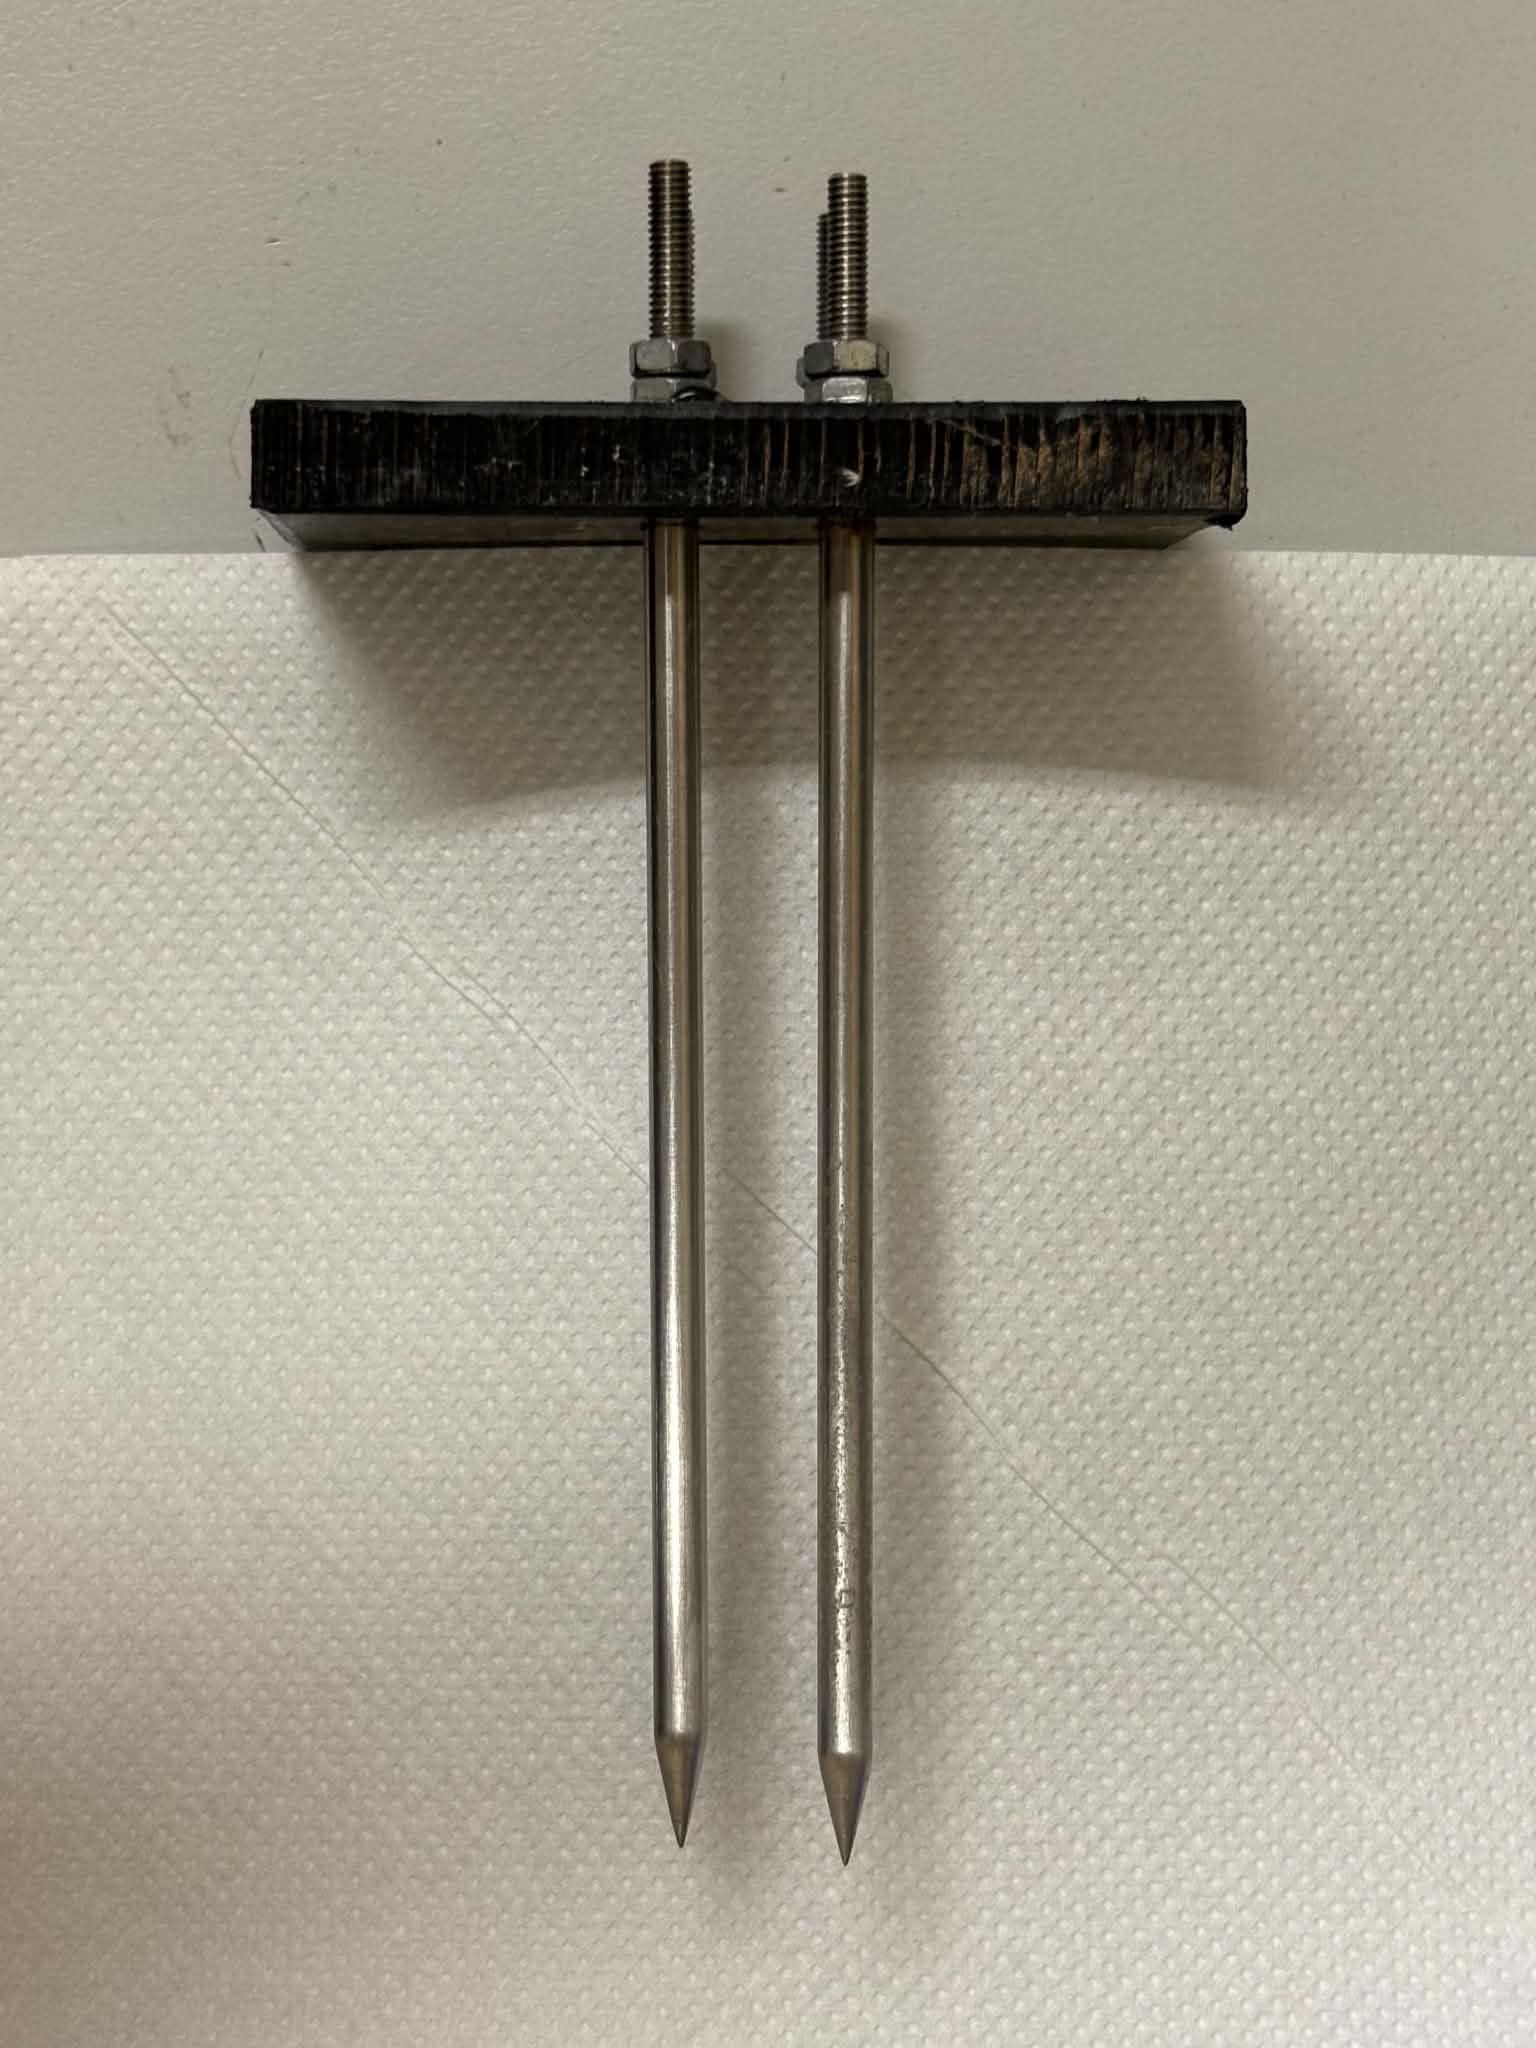
\includegraphics[width=0.5\textwidth]{figures/electrode.jpeg}
  \caption{Τα ηλεκτρόδια που χρησιμοποιήθηκαν κατά τα πειράματα.}
  \label{fig:signal-buffering-filtering}
\end{figure}




\section{Βαθμονόμιση}
 Ο αισθητήρας, αφού υπολογίσει τις εκτιμώμενες τιμές R και C του δείγματος, υπολογίζει αντίστοιχα τα \(\varepsilon_r'\) και \(\varepsilon_r''\). Όπως αναφέρθηκε στο Κεφάλαιο 2, οι αισθητήρες που καταφέρνουν να απομονώσουν το \(\varepsilon_r' \) υπολογίζουν με μεγαλύτερη ακριβεία την παρουσία και νερού. Ωστόσο, είτε σε χαμηλότερες συχνότητες είτε σε τύπους εδαφών που διαθέτουν υψηλή αλατότητα ο διαχωρισμός αυτός γίνεται δυσκολότερος λόγω της αυξημένης επίδρασης της αγωγιμότητας. Για το λόγο αυτό χρησιμοποιείται συχνά η φαινόμενη διηλεκτρική διαπερατότητα (apparent permittivity), η οποία συνδυάζει την επίδραση και των δύο συνιστωσών και ορίζεται ως \cite{ref19}

 \[
\varepsilon_a = \frac{\varepsilon_r'}{2}
\left(1 + \sqrt{1 + \left(\frac{\varepsilon_r''}{\varepsilon_r'}\right)^2}\right)
\tag{5.2}\]

Για τη βαθμονόμιση του αισθητήρα, πραγματοποιήθηκαν μετρήσεις σε δείγματα εδάφους τύπου Sandy Loam, τα οποία ξηράνθηκαν σε θερμοκρασία \(105\,^\circ \mathrm{C} \) για 10 ώρες. Τα δείγματα εξετάστηκαν από σχεδόν πλήρως ξηρή έως έντονα υγρή κατάσταση. Η υγρασία των δειγμάτων αυξανόταν σταδιακά με τη προσθήκη νερού και ακολουθούσε ομογενοποίηση του δείγματος προκειμένου να επιτευχθεί όσο το δυνατόν πιο ομοιόμορφη κατανομή της υγρασίας στο έδαφος.
\par Σε κάθε κατάσταση υγρασίας, πραγματοποιήθηκε επιπλέον μέτρηση με τον εμπορικό αισθητήρα TEROS 12. Πρόκειται για έναν αισθητήρα της METER Group ο οποίος υπολογίζει ογκομετρική περιεκτικότητα σε νερό, θερμοκρασία και η ηλεκτρική αγωγιμότητα εδάφους. Για τον υπολογισμό της υγρασίας χρησιμοποιεί τεχνολογία χωρητικής μέτρησης στα 70MHz και παρέχει ακρίβεια ±0.03 m3/m3 (±3.00\% VWC) στα ανόργανα εδάφη ηλεκτρικής αγωγιμότητας χαμηλότερης των 8,000 μS/cm \cite{ref47}.
\par Στα Σχήματα 5.2 και 5.3 φαίνονται στιγμιότυπα από τις μετρήσεις που πραγματοποιήθηκαν με τον αισθητήρα και το TEROS 12 αντίστοιχα.



\begin{figure}[H]
  \centering
  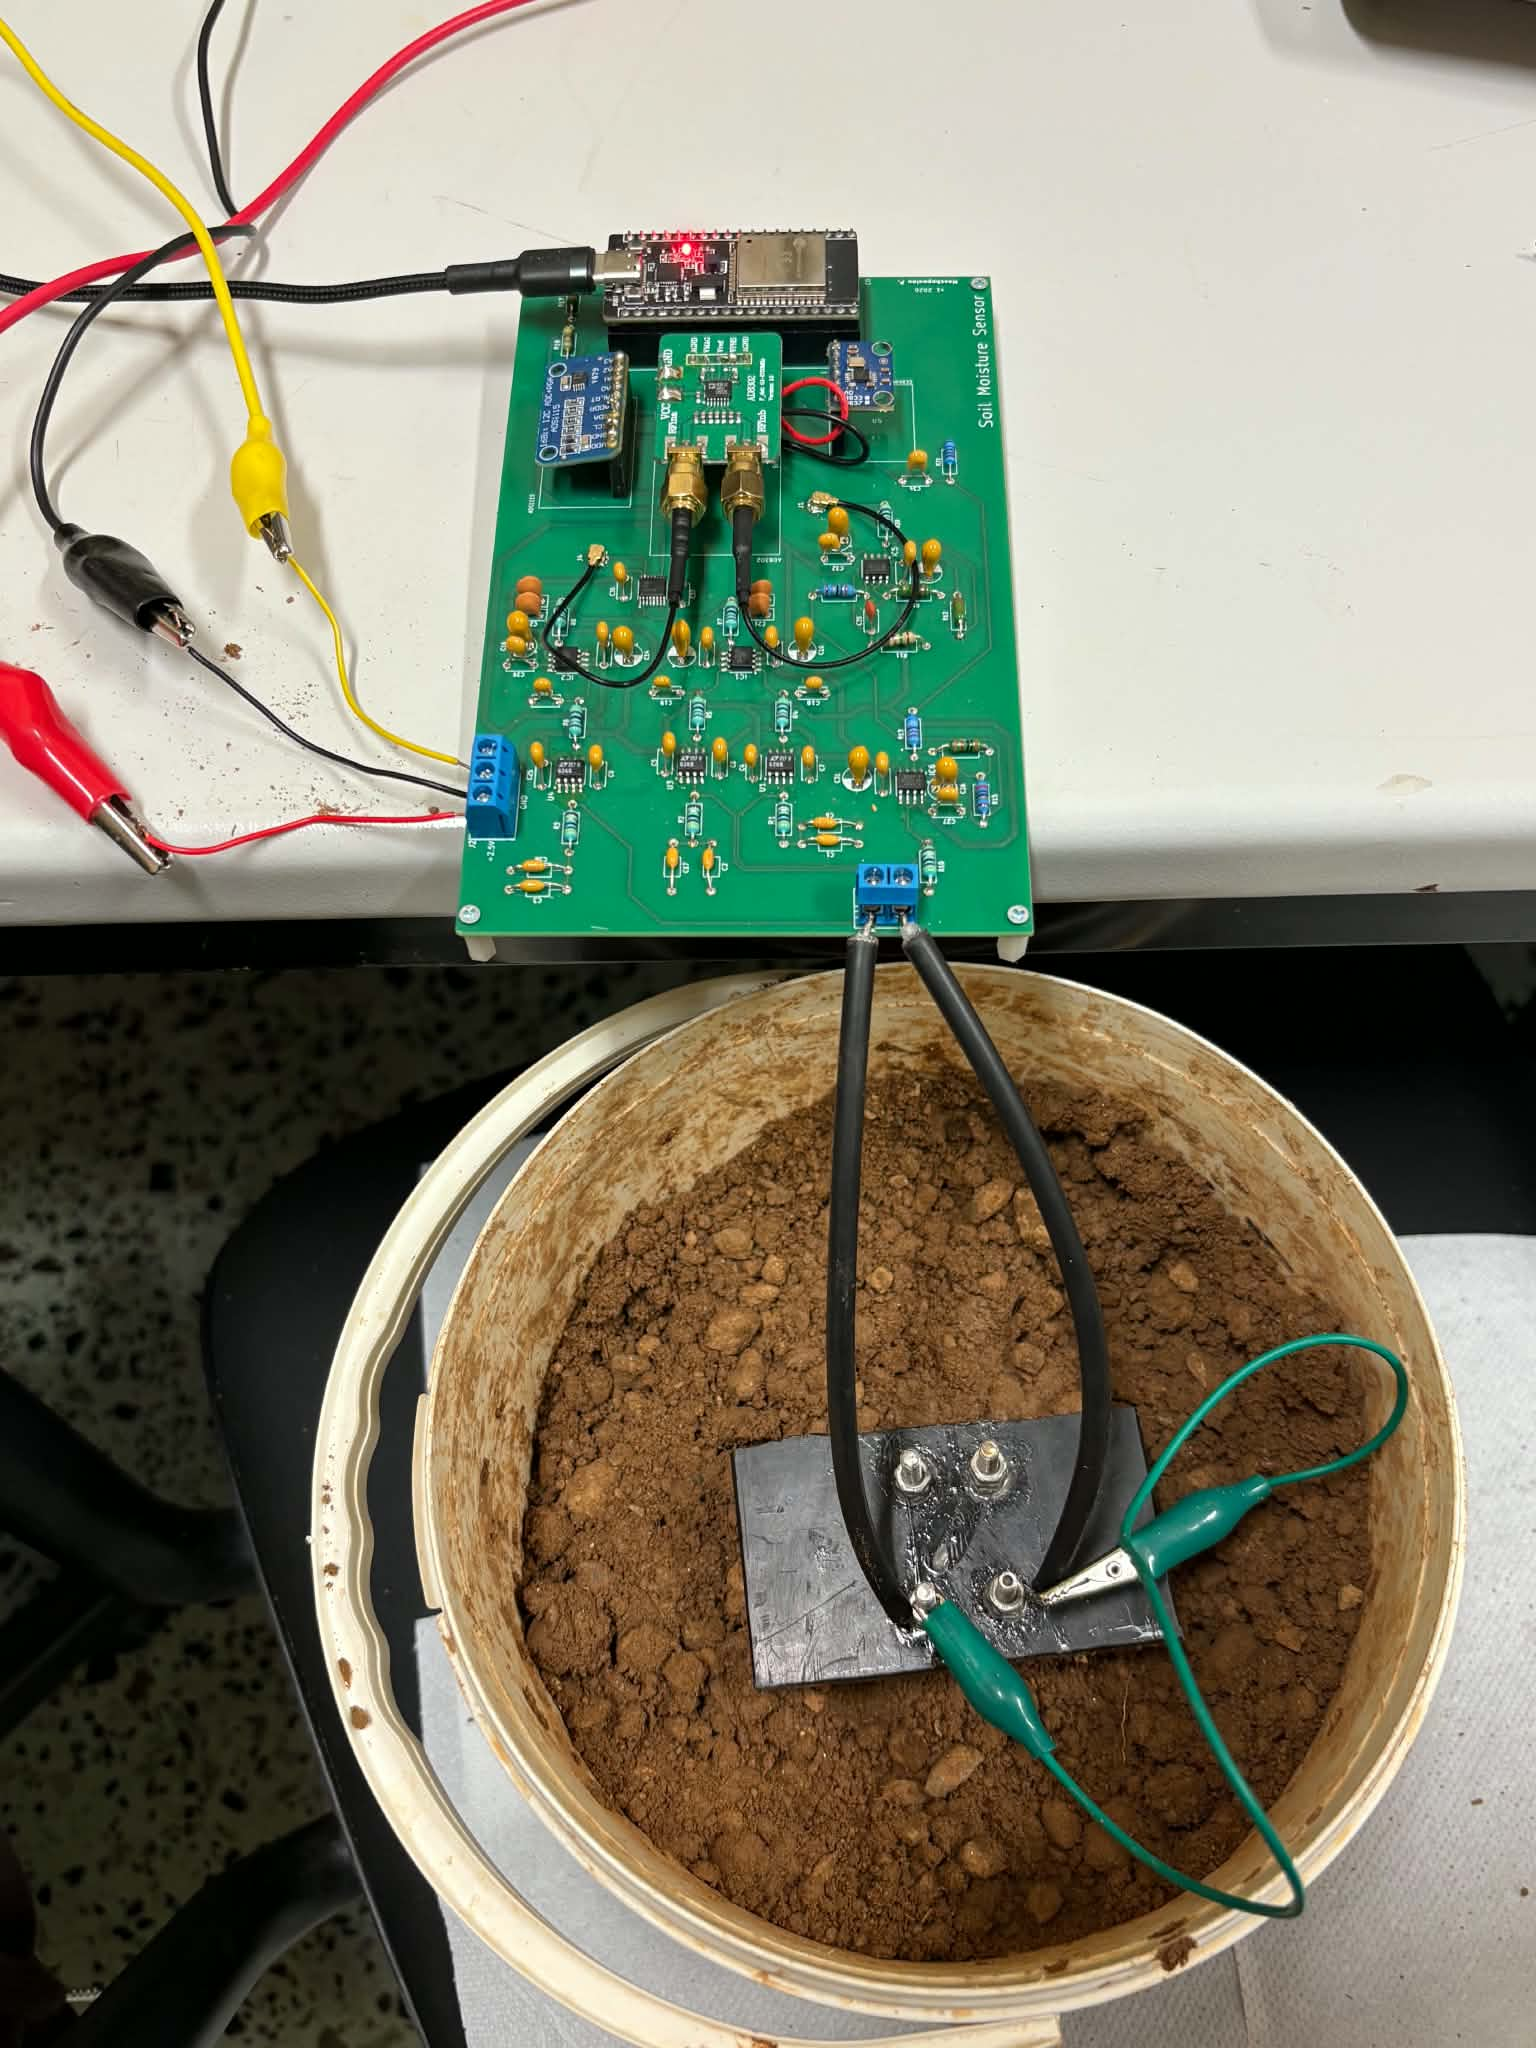
\includegraphics[width=0.45\textwidth]{figures/exp.jpeg}
  \caption{Στιγμιότυπο κατά τις πειραματικές μερήσεις με τον αισθητήρα.}
  \label{fig:signal-buffering-filtering}
\end{figure}

\begin{figure}[H]
  \centering
  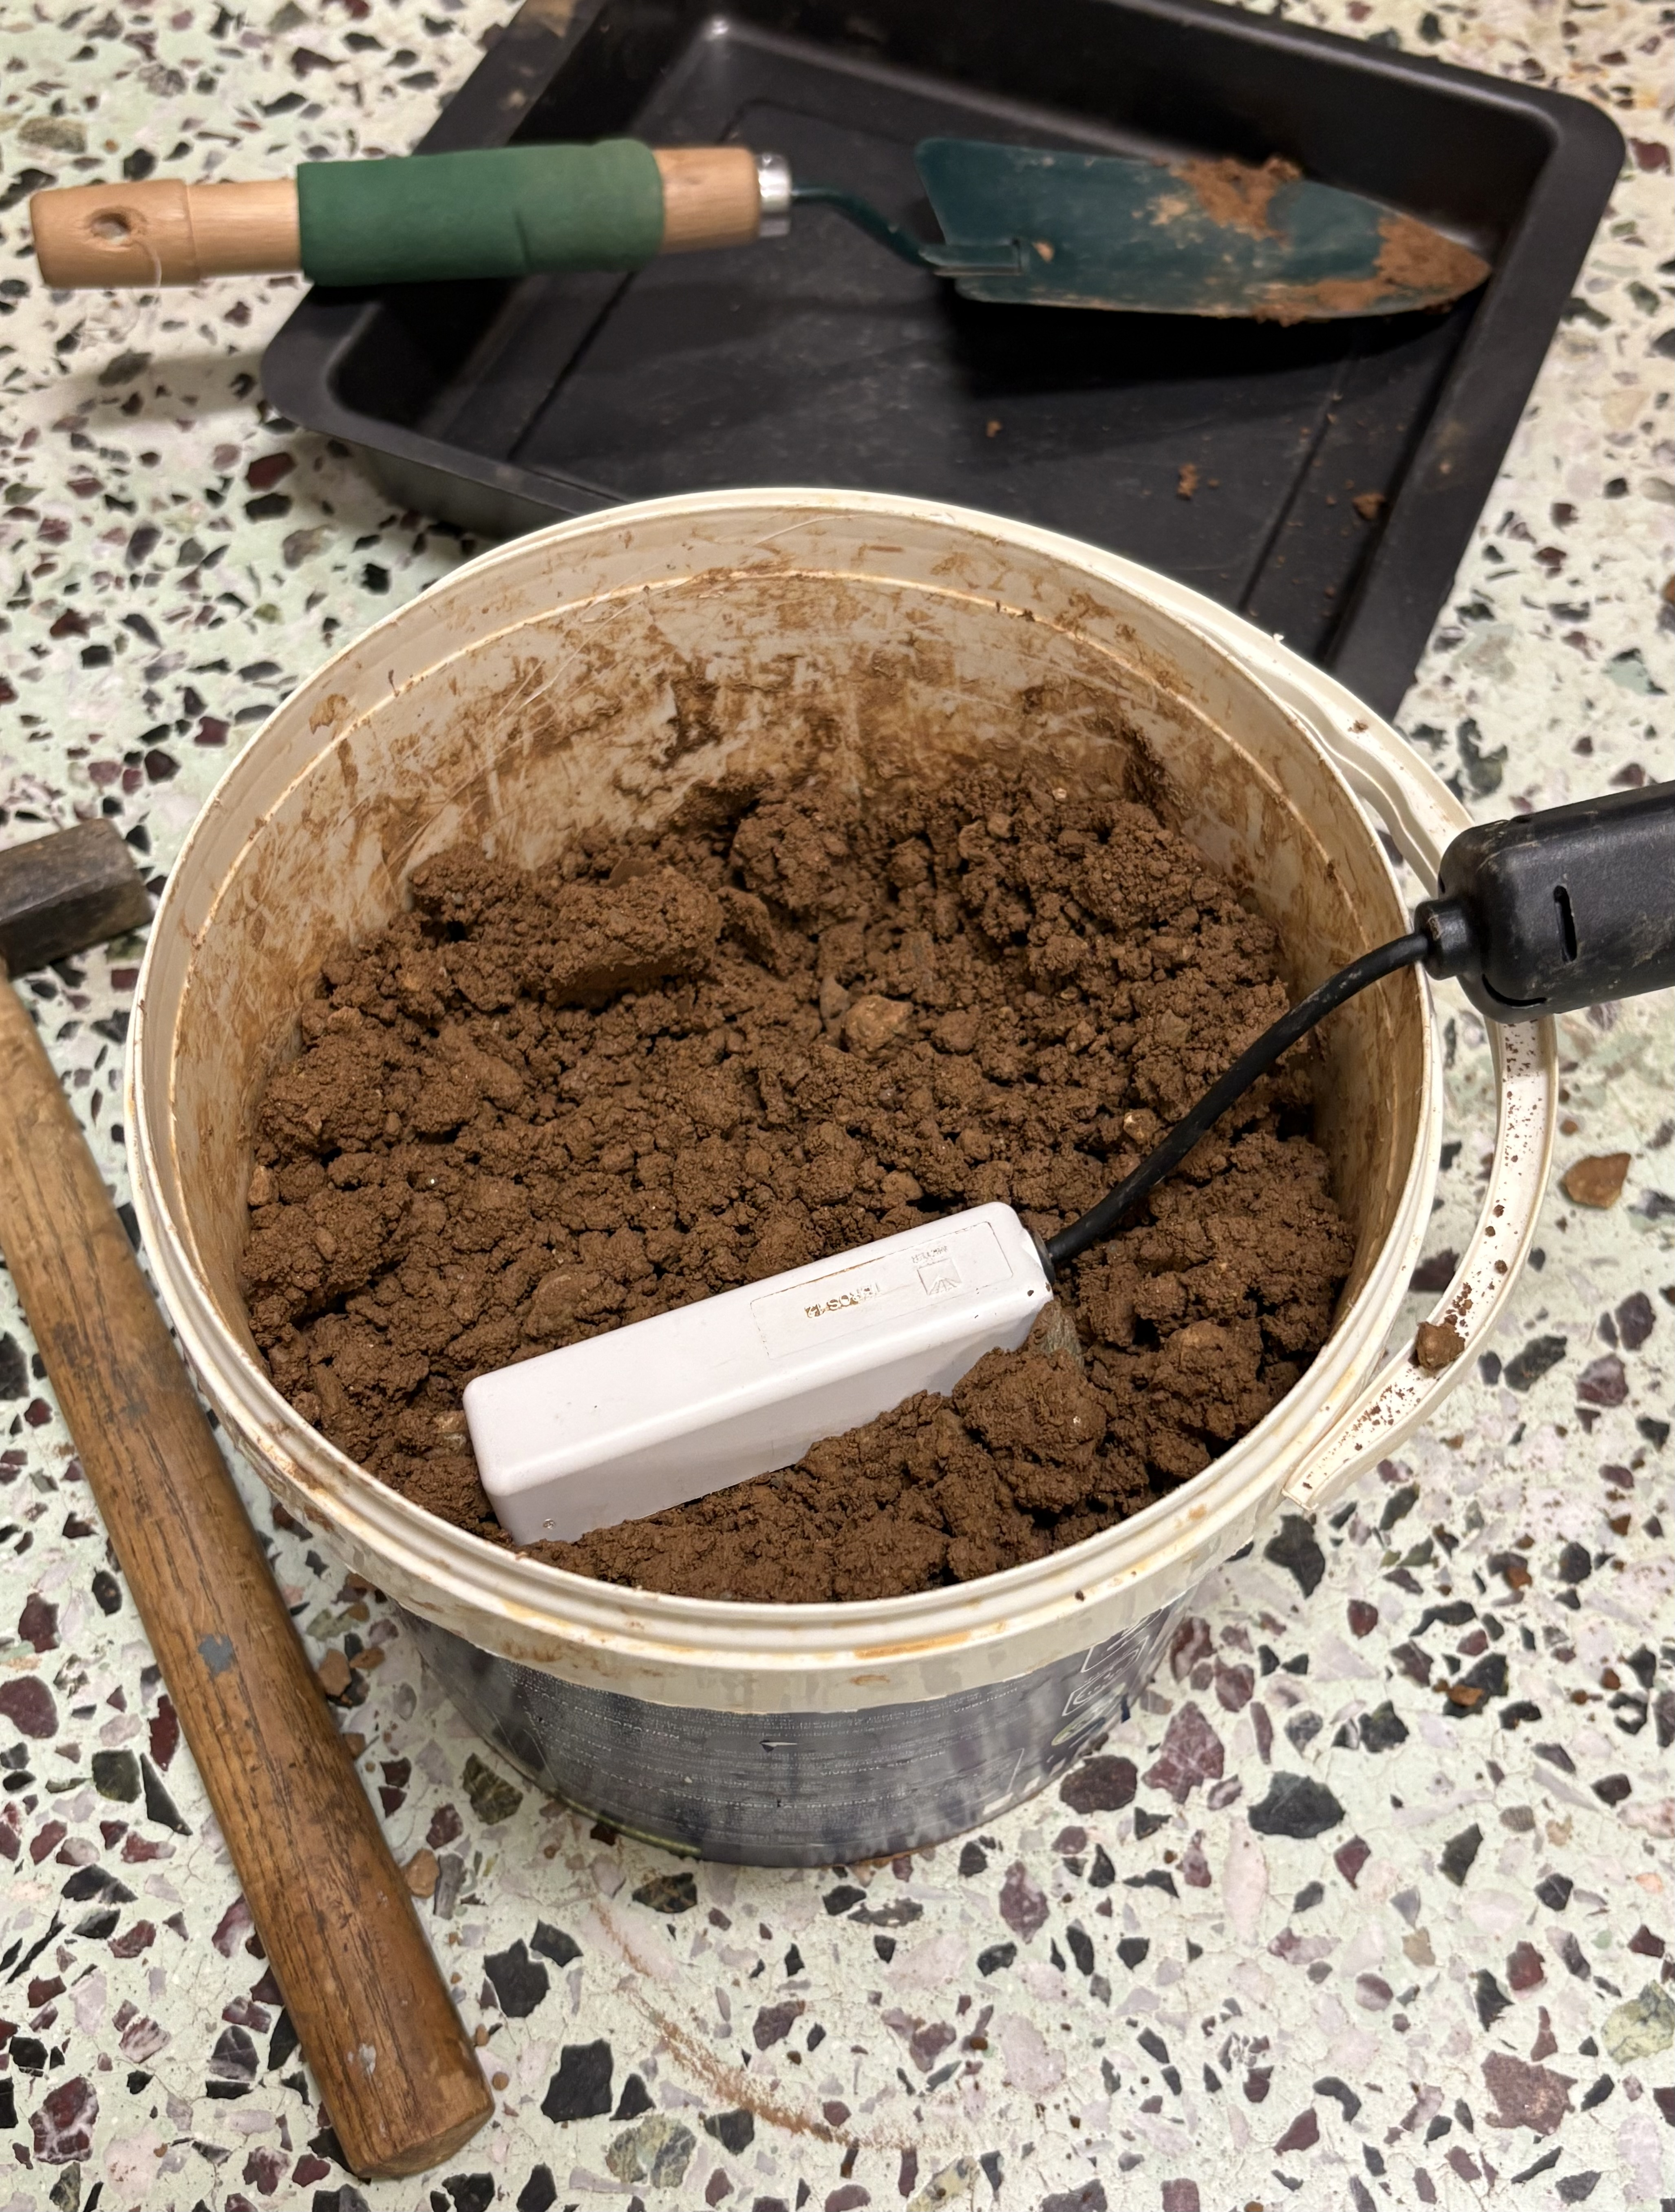
\includegraphics[width=0.45\textwidth]{figures/teros.jpg}
  \caption{Στιγμιότυπο κατά τις πειραματικές μερήσεις με το TEROS 12.}
  \label{fig:signal-buffering-filtering}
\end{figure}



\par Οι μετρήσεις των παραμέτρων $\varepsilon_r', \varepsilon_{\mathrm{apparent}}$ που υπολογίζει ο αισθητήρας χρησιμοποιήθηκαν για την αξιολόγηση των δύο μαθηματικών μοντέλων (23) και (24), προκειμένου να προσδιοριστεί ο συνδυασμός παραμέτρου κι εξίσωσης που παρουσιάζει το μικρότερο σφάλμα σε σχέση με τις τιμές αναφοράς θ του εμπορικού αισθητήρα.

\begin{align}
\theta &= a\sqrt{x} + b \tag{5.3}\\
\theta &= ax^3 + bx^2 + cx + d \tag{5.4}
\end{align}

 Αφού έγινε η προσαρμογή των πειραματικών δεδομένων $\varepsilon_r' \text{ και } \varepsilon_{\mathrm{apparent}}$ που προέκυψαν από τις μετρήσεις στις παραπάνω εξισώσεις, έγινε η αξιολόγηση του καταλληλότερου μοντέλου σύμφωνα με τις τιμές των \(R^2\) και RMSE που υπολογίστηκαν. 
 \par Τα μεγέθη αυτά ορίζονται αντίστοιχα ως

\[
\displaystyle
R^2 = 1 -
\dfrac{
\sum_{i=1}^{N} (y_i-\hat{y}_i)^2
}{
\sum_{i=1}^{N} (y_i-\bar{y})^2
}
\tag{5.5}\]

όπου \(N\) είναι ο συνολικός αριθμός μετρήσεων, \(y_i\) η πειραματική τιμή αναφοράς, \(\hat{y}_i\) η προβλεπόμενη τιμή του μοντέλου και \(\bar{y}\) η μέση τιμή των πειραματικών μετρήσεων, καθώς και 

\[
\displaystyle
\mathrm{RMSE} =
\sqrt{
\dfrac{1}{N}
\sum_{i=1}^{N}(y_i-\hat{y}_i)^2
}
\tag{5.6}\]

όπου \(N\) είναι ο συνολικός αριθμός μετρήσεων, \(y_i\) η πειραματική τιμή αναφοράς και \(\hat{y}_i\) η αντίστοιχη προβλεπόμενη τιμή του μοντέλου.
 
 \parΓια την εξαγωγή των καμπυλών και τον υπολογισμό των παραπάνω μεγεθών αξιολόγησης χρησιμοποιήθηκε η στατιστική γλώσσα προγραμματισμού R. Στα Σχήματα 5.3 έως 5.6  παρουσιάζονται οι καμπύλες που προκύπτουν μετά από την προσαρμογή, από τους συνδιασμούς των δύο παραμέτρων και των δύο μαθηματικών εξισώσεων που αποφασίσθηκε να δοκιμαστούν, ενώ στον πίνακα 5.1 συνοψίζονται οι τιμές \(R^2\) και RMSE για όλα τα μοντέλα.




% Τέσσερα σκρινσοτ




\begin{figure}[H]
  \centering
  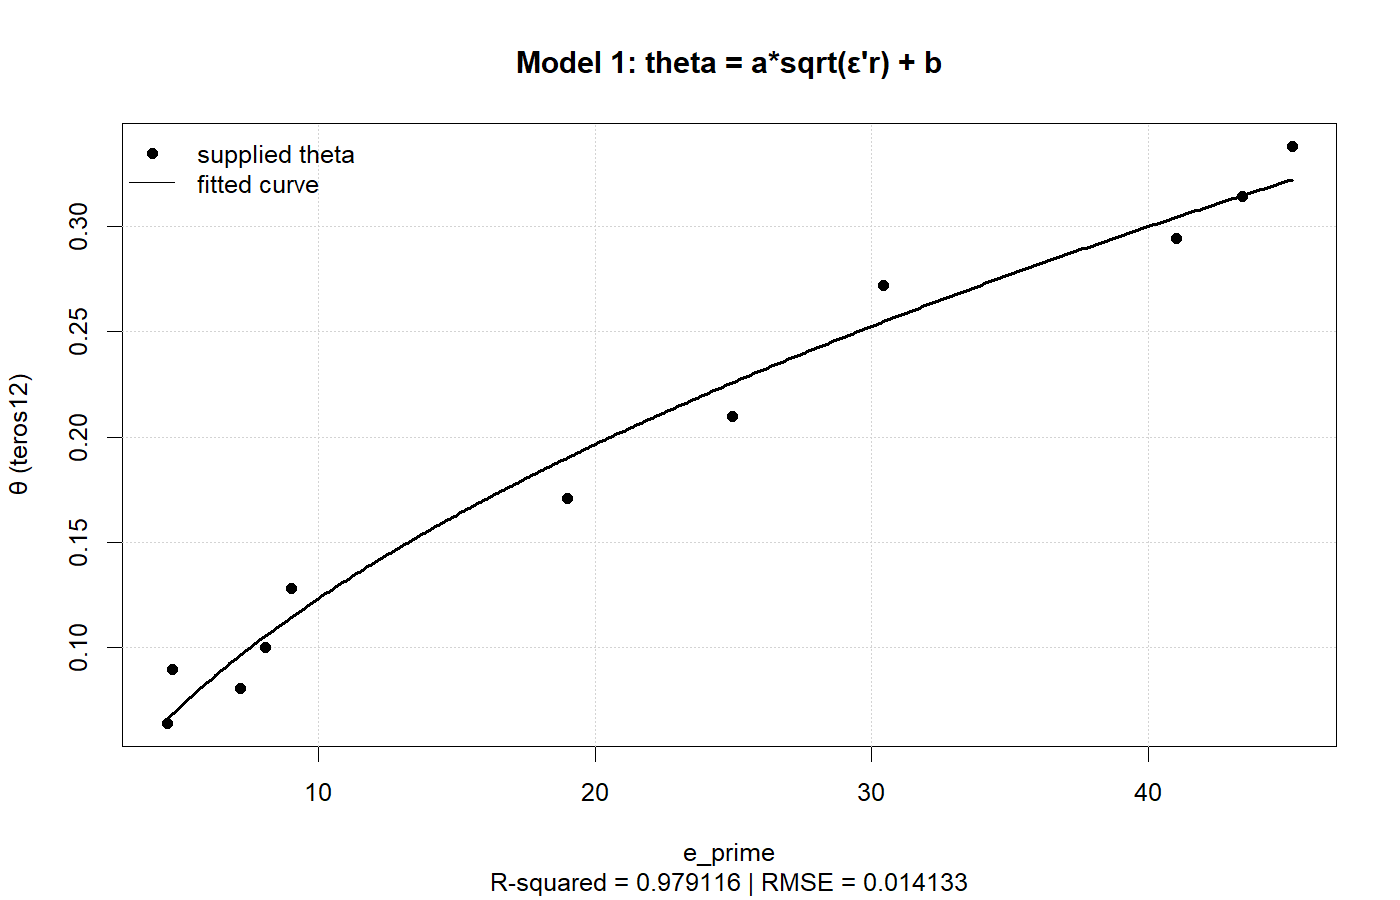
\includegraphics[width=0.99\textwidth]{figures/fit_1_sqrt_e_prime.png}
  \caption{Μοντέλο 1: Προσαρμογή της εξίσωσης (5.3) στα πειραματικά δεδομένα των γνωστών θ μέσω του TEROS12, προς την παράμετρο \(\varepsilon_r'\). Παρουσιάζεται η ποιότητα προσαρμογής του μοντέλου, μέσω των \(R^2 = 0{,}9791\) και RMSE \(= 0{,}0141\) (m³/m³) }
  \label{fig:signal-buffering-filtering}
\end{figure}




\begin{figure}[H]
  \centering
  \includegraphics[width=0.99\textwidth]{fit_2_sqrt_ea.png}
  \caption{Μοντέλο 2: Προσαρμογή της εξίσωσης (5.3) στα πειραματικά δεδομένα των γνωστών θ μέσω του TEROS12, προς την παράμετρο \(\varepsilon_a\). Παρουσιάζεται η ποιότητα προσαρμογής του μοντέλου, μέσω των \(R^2 = 0{,}9724\) και RMSE \(= 0{,}0162\) (m³/m³) }
  \label{fig:signal-buffering-filtering}
\end{figure}


\begin{figure}[H]
  \centering
  \includegraphics[width=0.99\textwidth]{fit_3_cubic_e_prime.png}
  \caption{Μοντέλο 3: Προσαρμογή της εξίσωσης (5.4) στα πειραματικά δεδομένα των γνωστών θ μέσω του TEROS12, προς την παράμετρο \(\varepsilon_r'\). Παρουσιάζεται η ποιότητα προσαρμογής του μοντέλου, μέσω των \(R^2 = 0{,}9831\) και RMSE \(= 0{,}0127\) (m³/m³) }
  \label{fig:signal-buffering-filtering}
\end{figure}



\begin{figure}[H]
  \centering
  \includegraphics[width=0.99\textwidth]{fit_4_cubic_ea.png}
  \caption{Μοντέλο 4: Προσαρμογή της εξίσωσης (5.4) στα πειραματικά δεδομένα των γνωστών θ μέσω του TEROS12, προς την παράμετρο \(\varepsilon_a\). Παρουσιάζεται η ποιότητα προσαρμογής του μοντέλου, μέσω των \(R^2 = 0{,}9938\) και RMSE \(= 0{,}0077\) (m³/m³) }
  \label{fig:signal-buffering-filtering}
\end{figure}


\begin{table}[H]
    \centering

    \renewcommand{\arraystretch}{0.8}
    \setlength{\tabcolsep}{45pt}

    \resizebox{\textwidth}{!}{%
    \begin{tabular}{lcc}
        \hline
        \textbf{Μοντέλο} & \textbf{$R^2$} & \textbf{RMSE} \\
        \hline
        Μοντέλο 1 & 0.979116 & 0.014133 \\
        Μοντέλο 2 & 0.972479 & 0.016224 \\
        Μοντέλο 3 & 0.983120 & 0.012706 \\
        Μοντέλο 4 & 0.993830 & 0.007682 \\
        \hline
    \end{tabular}%
    }

    \caption{Σύγκριση των μοντέλων προσαρμογής βάσει των
    δεικτών $R^2$ και RMSE (m³/m³).}
    \label{tab:model_comparison}
\end{table}


\par Έπειτα από τη δοκιμή και αξιολόγηση των παραπάνω συναρτήσεων προσαρμογής μέσω επαναλλειπτικών μετρήσεων, διαπιστώνεται πως η πολυωνυμική εξίσωση τρίτου βαθμού με παράμετρο το \(\varepsilon_{a}\) παρουσιάζει την καλύτερη συνολική συμπεριφορά ως προς την ακρίβεια προσαρμογής. Στην εξίσωση 5.7 παρουσιάζονται οι συντελεστές της εξίσωσης

\[
\theta = -5.20 \times 10^{-10}x^3 + 8.56 \times 10^{-8}x^2 + 0.000602x + 0.061913
\tag{5.7}\]









\chapter{Ανάπτυξη Firmware και Διασύνδεση με το Cloud}
\label{ch:firmware}

\section{Εισαγωγή}
Η ανάπτυξη του λογισμικού του συστήματος αποτέλεσε βασικό στάδιο για την ολοκλήρωση της λειτουργίας του αισθητήρα. Μέσω του μικροελεγκτή έγινε η διαχείρηση των επιμέρους μονάδων, η εφαρμογή της μαθηματικής λογικής για την επεξεργασία των μετρήσεων, καθώς και η σύνδεση του συστήματος στο διαδίκτυο για την απεικόνιση των μετρήσεων στο Cloud. Στο παρόν κεφάλαιο περιγράφεται η δομή και η λειτουργία του λογισμικού που αναπτύχθηκε.



\section{Firmware}
Η ανάπτυξη του κώδικα έγινε στο προγραμματιστικό περιβάλλον Visual Studio Code με τη χρήση της επέκτασης PlatformIO σε γλώσσα προγραμματισμού C++. Στην εικόνοα τάδε φαίνεται το διάγραμμα ροής της λειτουργίας του συστήματος.

\par Πιο συγκεκριμένα, κατά την εκκίνηση του συστήματος γίνεται η αρχικοποίηση των διάφορων περιφερειακών που χρησιμοποιούνται για τη λήψη και επεξεργασία των μετρήσεων, χρησιμοποιώντας τις κατάλληλες βιβλιοθήκες. Συγκεκριμένα, για τον έλεγχο της γεννήτριας σημάτων AD9833 ορίζεται η συχνότητα και ο τύπος της κυματομορφής εξόδου μέσω του διαύλου SPI . Επιπλέον, αρχικοποιείται ο μετατροπέας αναλογικού σε ψηφιακό σήμα ο οποίος επικοινωνεί με το μικροελεγκτή μέσω του διαύλου I2C.

\par Επιπλέον, ορίζονται οι συναρτήσεις με τη βοήθεια των οποίων θα γίνει η σύνδεση στο διαδίκτυο με τη χρήση της βιβλιοθήκης WiFiManager, ενώ γίνεται και χρήση της μη πτητικής μνήμης του μικροελεγτκή μέσω της βιβλιοθήκης Preferences προκειμένου να αποθηκεύονται γνωστά τοπικά δίκτυα τα οποία εισάγει ο χρήστης. Κατά τη διαδικασία της σύνδεσης, ο μικροελεγτκής αναζητά διαθέσιμα δίκτυα κι επιχειρεί να συνδεθεί σε κάποιο ήδη αποθηκευμένο. Εφόσον δεν τα καταφέρει, ενεργοποιείται ένα ενεργό σημείο πρόσβασης (access point), μέσω του οποίου ο χρήστης μπορεί να συνδεθεί από τον υπολογιστή ή το κινητό και να επιλέξει το επιθυμητό δίκτυο, εισάγοντας τον αντίστοιχο κωδικό πρόσβασης. Τα στοιχεία αυτά αποθηκεύονται αυτόματα στη μη πτητική μνήμη του μικροελεγκτή. Μετά την επιτυχή σύνδεση, αρχικοποιείται η σύνδεση με το Arduino Cloud για την αποστολή των μετρήσεων.

\par Στο εσωτερικό της συνάρτησης loop() εκτελείται επαναλαμβανόμενα η λήψη κι επεξεργασία των μετρήσεων. Αρχικά, λαμβάνεται μέσω του ADC η DC έξοδος του AD8302 για το πρώτο ζεύγος τιμών στην είσοδό του, ενώ στη συνέχεια αλλάζει η κατάσταση του αναλογικού διακόπτη  μέσω του μικροελεγτκή και λαμβάνεται η τιμή εξόδου για το δεύτερο ζεύγος τιμών. Στη συνέχεια υλοποιείται η μαθηματική λογική για τον υπολογισμό των παραμέτρων $R$, $C$, $\varepsilon'_r$, $\varepsilon''_r$, $\varepsilon_{\mathrm{apparent}}$ και μέσω της εξίσωσης βαθμονόμισης υπολογίζεται τελικά η ογκομετρική υγρασία. Τέλος, οι μετρήσεις αποστέλλονται στο Arduino Cloud.


\section{ Arduino Cloud}
Για την απεικόνιση των μετρήσεων χρησιμοποιήθηκε η πλατφόρμα Arduino Cloud, η οποία μέσω της διαδυκτιακής σύνδεσης προσφέρει απομακρυσμένo έλεγχο και παρακολούθηση των μετρήσεων μέσω συμβατών μικροελεγκτών. Προσφέρει τη δυνατότητα συλλογής και απεικόνισης δεδομένων σε πραγματικό χρόνο, ενώ προσφέρει και τη δυνατότητα διατήρησης ιστορικού για την ανάλυση των  μετρήσεων σε βάθος χρόνου. Στην εικόνα τάδε φαίνεται το dashboard που υλοποιήθηκε για την παρακολούθηση των δεδομένων. Ο χρόνος που έχει οριστεί προγραμματιστικά να ενημερώνονται οι μεταβλητές είναι τα τόσα λεπτά.






\chapter{Συμπεράσματα και Βελτιώσεις}
\label{ch:end}

\section{Εισαγωγή}
Στο παρόν κεφάλαιο παρουσιάζεται η πειραματική αξιολόγηση του αισθητήρα. Αρχικά, εξετάζεται η συμπεριφορά του αισθητήρα κατά τη μεταβολή της υγρασίας και παρουσιάζονται τα αποτελέσματα συγκριτικά με τον αισθητήρα αναφοράς TEROS 12. Τέλος, συνοψίζονται τα βασικά συμπεράσματα για τον αισθητήρα που αναπτύχθηκε, οι περιορισμοί, καθώς και μελλοντικές βελτιώσεις για την εξέλιξη του συστήματος.

\section{Αξιολόγηση}
Για την αξιολόγηση του αισθητήρα επαναλήφθηκε το πείραμα από πολύ ξηρό έως έντονα υγρό δείγμα εδάφους και λήφθηκαν μετρήσεις τόσο από τον αισθητήρα όσο και από το TEROS 12. Στον πίνακα 7.1 παρουσιάζεται το σύνολο τιμών από την πρώτη πειραματική αξιολόγηση του αισθητήρα συγκριτικά με τις μετρήσεις του εμπορικού αισθητήρα.

\par Επιπλέον, υπολογίζεται το Μέσο Απόλυτο Σφάλμα το οποίο εκφράζει τη μέση απόλυτη διαφορά μεταξύ των μετρήσεων των δύο αισθητήρων και ορίζεται ως

\[
MAE = \frac{1}{n}\sum_{i=1}^{n}\left|S_i - T_i\right|
\tag{7.1}\]

όπου n το πλήθος των μετρήσεων, \(S_i\) η μέτρηση του αισθητήρα, \(T_i\) η μέτρηση αναφοράς του TEROS12 και \(\left|S_i-T_i\right|\) η απόλυτη διαφορά μεταξύ των δύο μετρήσεων.



\begin{table}[H]
    \centering
    \begin{tabularx}{\textwidth}{
        *{8}{>{\centering\arraybackslash}X}
    }
        \toprule
        $\theta_{\text{sensor}}$ & 0.077 & 0.098 & 0.121 & 0.157 & 0.211 & 0.236 & 0.340 \\
        \cmidrule(lr){2-8}
        $\theta_{\text{TEROS}}$ & 0.078 & 0.094 & 0.119 & 0.155 & 0.232 & 0.271 & 0.304 \\
        \bottomrule
    \end{tabularx}
    \caption{Σύγκριση μετρήσεων ογκομετρικής υγρασίας μεταξύ του αισθητήρα και του εμπορικού TEROS 12.}
    \label{tab:measurements}
\end{table}


\par Η μέγιστη απόλυτη διαφορά μεταξύ των μετρήσεων των δύο αισθητήρων είναι 0.036 \(\mathrm{m^3/m^3}\) ή 3.6 ποσοστιαίες μονάδες ογκομετρικής υγρασίας. Το Μέσο Απόλυτο Σφάλμα όπως προκύπτει από τον τύπο 7.1 και υπολογίζεται στα 0.0144 \(\mathrm{m^3/m^3}\) ή 1.44 ποσοστιαίες μονάδες ογκομετρικής περιεκτικότητας σε νερό.


\par Το πείραμα επαναλήφθηκε με παραπάνω δείγματα και βελτιωμένες πειραματικές συνθήκες ομογενοποιώντας
καλύτερα το δείγμα, αφήνοντας τα ηλεκτρόδια των δύο αισθητήρων στο έδαφος να πλησιάσουν τη θερμοκρασία του δείγματος 
και λαμβάνοντας το μέσο όρο πολλών μετρήσεων για κάθε δείγμα. Τα αποτελέσματα παρουσίαζονται στον 
πίνακα 7.2, υπολογίζοντας και το Σχετικό Σφάλμα ως

\[
E_{\mathrm{rel},i}(\%)=
\frac{|S_i-T_i|}{T_i}\times100
\tag{7.2}\]



\begin{table}[H]
    \centering
    \small
    \setlength{\tabcolsep}{3pt}
    \begin{tabularx}{\textwidth}{
        >{\centering\arraybackslash}p{2.5cm}
        *{11}{>{\centering\arraybackslash}X}
    }
        \toprule
        $\theta_{\text{sensor}}$
        & 0.055 & 0.071 & 0.083 & 0.110 & 0.132 & 0.181
        & 0.234 & 0.270 & 0.312 & 0.318 & 0.320 \\
        \cmidrule(lr){2-12}
        $\theta_{\text{TEROS}}$
        & 0.064 & 0.081 & 0.090 & 0.100 & 0.128 & 0.171
        & 0.210 & 0.272 & 0.294 & 0.314 & 0.338 \\
        \midrule
        {\scriptsize Απόλυτη Διαφορά}
        & 0.009 & 0.010 & 0.007 & 0.010 & 0.004 & 0.010
        & 0.024 & 0.002 & 0.018 & 0.004 & 0.018 \\
        \midrule
        {\scriptsize Σχετικό Σφάλμα (\%)}
        & 14.06 & 12.35 & 7.78 & 10.00 & 3.13 & 5.85
        & 11.43 & 0.74 & 6.12 & 1.27 & 5.33 \\
        \bottomrule
    \end{tabularx}
    \caption{Σύγκριση μετρήσεων ογκομετρικής υγρασίας μεταξύ του αισθητήρα και του εμπορικού TEROS 12, με την απόλυτη διαφορά και το σχετικό σφάλμα ανά ζεύγος μετρήσεων.}
    \label{tab:measurements}
\end{table}



\par Το Μέσο Απόλυτο Σφάλμα υπολογίζεται στο 0.0105 \(\mathrm{m^3/m^3}\), τιμή η οποία αντιστοιχεί σε  1.05 ποσοστιαία μονάδα ογκομετρικής περιεκτικότητας σε νερό, το Μέσο Σχετικό Σφάλμα υπολογίζεται στα 7.1\% ενώ το Μέγιστο Σχετικό Σφάλμα που εμφανίζεται είναι 14.06\%




Για την οπτικοποίηση των αποτελεσμάτων του τελευταίου πειράματος, παρατίθεται το διάγραμμα διασποράς στο Σχήμα 7.1 μέσω της σύγκρισης των δύο αισθητήρων. Πρόκειται για ένα διάγραμμα που χρησιμοποιεί σημεία για να συγκρίνει πόσο κοντά βρίσκονται δύο σύνολα μετρήσεων. Συγκεκριμένα, για κάθε μέτρηση δημιουργείται ένα ζεύγος σημείων
με συντεταγμένες $(x,y) = (\theta_{\mathrm{TEROS12}},
\theta_{\mathrm{sensor}})$. Η κόκκινη γραμμή απεικονίζει τη
γραμμή ιδανικής συμφωνίας και λειτουργεί ως αναφορά, καθώς όσο πιο κοντά σε αυτή βρίσκονται τα σημεία τόσο μικρότερη είναι η διαφορά στη μέτρηση.


\begin{figure}[H]
  \centering
  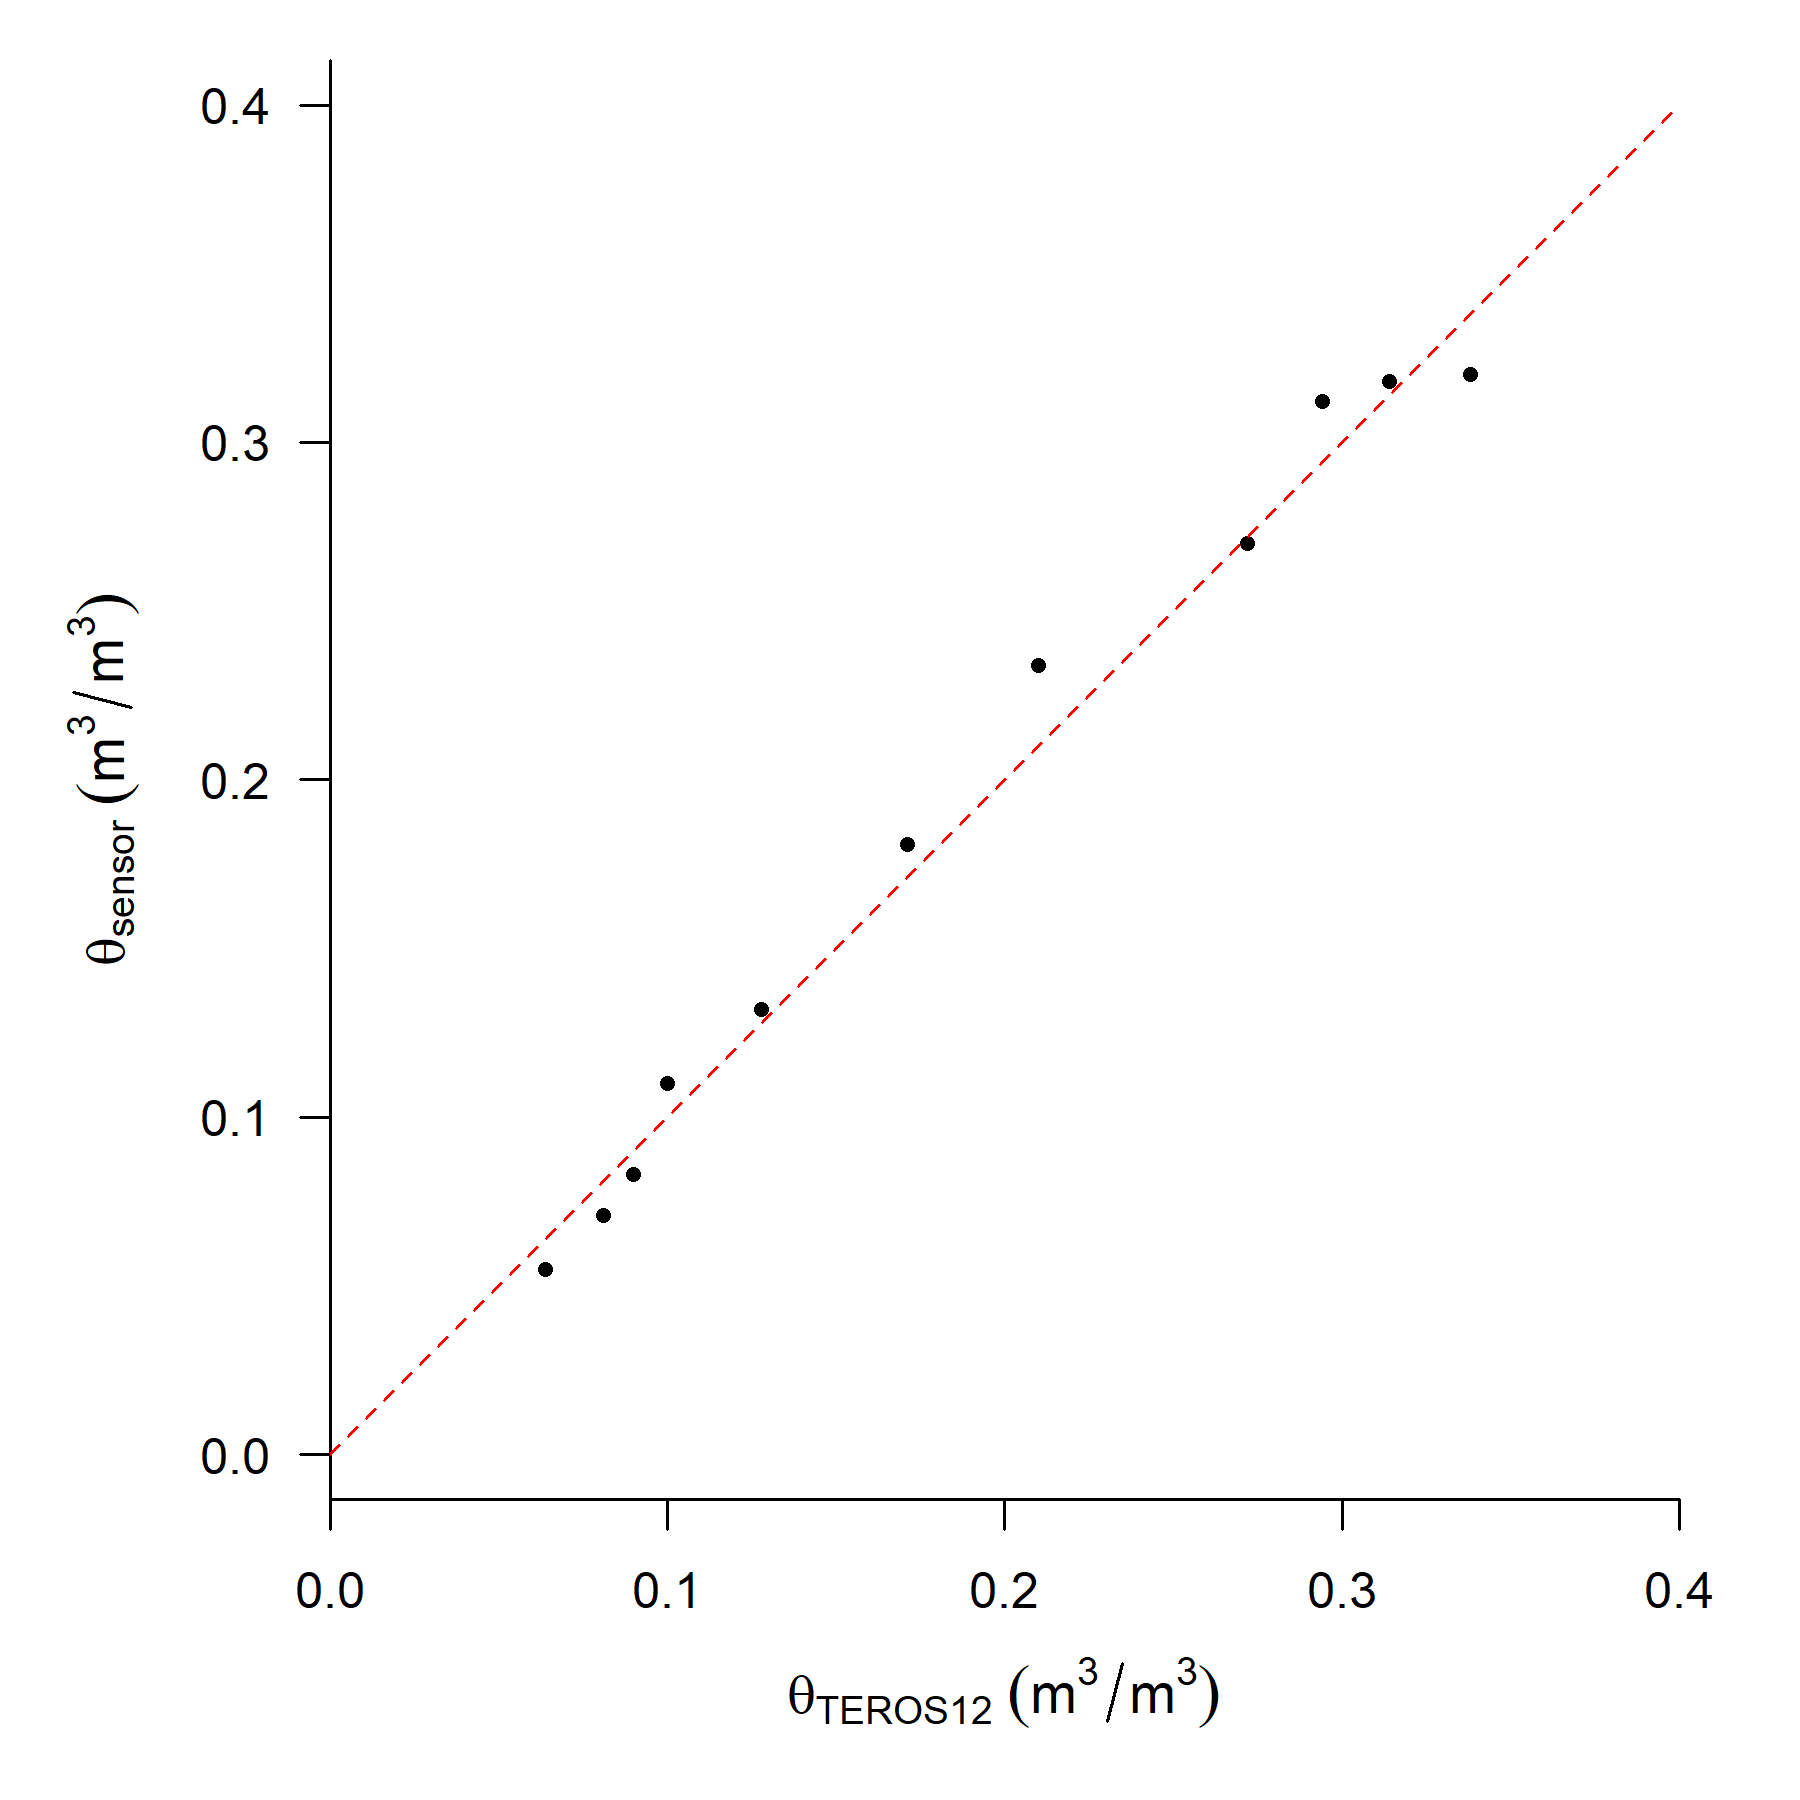
\includegraphics[width=0.65\textwidth]{figures/sensor_vs_teros.png}
  \caption{Το διάγραμμα διασποράς για τα ζεύγη μετρήσεων του αισθητήρα και του TEROS 12.}
  \label{fig:signal-buffering-filtering}
\end{figure}


Παρατηρείται ότι για τιμές ογκομετρικής υγρασίας κοντά στο \(0{,}32\ \mathrm{m^3/m^3}\) υπάρχει μία σταθεροποίηση των τιμών εξόδου των αισθητήρων. Το φαινόμενο αυτό οφείλεται σε διάφορους παράγοντες όπως ενδεχομένως τον κορεσμό του εδάφους, η κατάσταση κατά την οποία σε όλους τους πόρους του εδάφους έχει διοχετευθεί νερό, αλλά και τη συσσώρευση ελεύθερου νερού που δε μπορεί να δεσμευθεί στην επιφάνεια του δείγματος. Η τιμή αυτή εξαρτάται από τις ιδιότητες του εδάφους και είναι διαφορετική ανάλογα με το πορώδες και τη δυνατότητα συγκράτησης νερού.


\section{Συμπεράσματα}
Στόχος της διπλωματικής αποτέλεσε η ανάπτυξη ενός αισθητήρα υγρασίας εδάφους σχετικά χαμηλού κόστους και πολυπλοκότητας, αξιόλογης όμως ακρίβειας συγκριτικά με έναν εμπορικό αισθητήρα. Με βάση τα αποτελέσματα της πειραματικής αξιολόγησης, ο αισθητήρας παρουσιάζει ικανοποιητική συμπεριφορά για το τύπο εδάφους στον οποίο έγινε η βαθονόμιση. Το γεγονός αυτό υποστηρίζει την ορθότητα της σχεδιαστικής προσέγγισης του συστήματος που αναπτύχθηκε αλλά και του θεωρητικού υποβάθρου που χρησιμοποιήθηκε για την υλοποίηση.

\par Η αξιολόγιση του αισθητήρα σε σύγκριση με τον αισθητήρα αναφοράς, οδήγησε στον υπολογισμό του μέσου απόλυτου σφάλματος του συστήματος υπό τις συνθήκες όπου υλοποιήθηκε και υπολογίζεται περίπου στα υπολογίστηκε περίπου στο
\(0{,}0105\ \mathrm{m^3/m^3}\) . Το μέγεθος αυτό αποτελεί έναν ενδεικτικό δείκτη για την εκτίμηση της μέσης απόκλισης του αισθητήρα σε σχέση με τον αισθητήρα αναφοράς.





\section{Βελτιώσεις}

\parΓια την ολοκληρωμένη διαμόρφωση του αισθητήρα είναι απαραίτητη η βαθμονόμιση και αξιολόγηση της συμπεριφοράς του σε διαφορετικούς τύπους εδαφών. Οι ιδιότητες του εδάφους όπως η κοκκομετρική σύσταση και η αλατότητα μπορούν να επηρεάσουν την ηλεκτρική απόκριση του αισθητήρα. Έτσι, κρίνεται αναγκαία η μελέτη δειγμάτων διαφορετικών κατηγοριών και η εξαγωγή των αντίστοιχων καμπυλών βαθμονόμισης ανάλογα με τις εδαφικές συνθήκες. Η διαδικασία αυτή θα επιτρέψει τη γενικευμένη χρήση του αισθητήρα, αλλά και θα εξασφαλίσει τη μέγιστη δυνατή ακρίβεια ανάλογα με τον τύπο εδάφους που θα ορίζει ο χρήστης.

\par Σημαντικό βήμα για την αξιοπιστία του αισθητήρα αποτελεί η βαθμονόμισή του σύμφωνα με το θεωρητικό υπολογισμό του ποσοστού της ογκομετρικής υγρασίας που περιέχεται στο δείγμα. Η διαδικασία αυτή συμβάλλει στην αυτονομία και την περαιτέρω εγκυρότητα των μετρήσεων του αισθητήρα υιοθετώντας μία πιο καθολική προσέγγιση και μειώνοντας παράλληλα τις αποκλίσεις που εισάγονται από τον εμπορικό αισθητήρα.

\par Χρήσιμη αναβάθμιση του αισθητήρα αποτελεί η μελέτη της κατανάλωσης του συστήματος και η ανάπτυξη αυτόνομης τροφοδοσίας, μέσω επαναφορτιζόμενης μπαταρίας και αυτόματης φόρτησης με τη χρήση ηλιακού πάνελ. Παράλληλα, η ενσωμάτωση τεχνικών για την εξοικονόμηση ενέργειας, όπως η λειτουργία χαμηλής κατανάλωσης μεταξύ των μετρήσεων τόσο στο ψηφιακό όσο και στο αναλογικό κομμάτι θα αυξήσει σημαντικά την αυτονομία του αισθητήρα. Με αυτό τον τρόπο, ο αισθητήρας θα μπορεί να λειτουργεί απομακρυσμένα και θα  περιοριστεί σημαντικά η ανάγκη για ανθρώπινη παρέμβαση.

\par Για την πιο συμπαγή κατασκευή του αισθητήρα είναι σημαντικός ο επανασχεδιασμός της πλακέτας. Η πυκνότερη τοποθέτηση των εξαρτημάτων, αλλά και η χρήση SMD στοιχείων θα βοηθήσει στη φορητότητα του αισθητήρα. Επιπλέον, μέσω της χρήσης τεσσάρων επιπέδων (4-layer PCB) και της τοποθέτησης των τροφοδοσιών σε ξεχωριστά επίπεδα, θα βελτιωθεί σημαντικά η εξοικονόμιση χώρου αλλά και η μείωση του θορύβου.

\par Μια βελτιωμένη έκδοση του αισθητήρα αποτελεί η λειτουργία του με σήμα διέγερσης υψηλότερης συχνότητας, ή εναλλακτικά σε φάσμα διαφορετικών συχνοτήτων για την καλύτερη απομόνωση του πραγματικού μέρους της διηλεκτρικής σταθεράς. Η προσέγγιση αυτή θα μπορούσε να συμβάλει στον ακριβέστερο υπολογισμό της υγρασίας, καθώς διευκολύνεται ο διαχωρισμός της παρουσίας νερού από άλλα εδαφικά χαρακτηριστικά.
